\documentclass[10pt]{book}

\usepackage{cdt/cdtUsecases}
\usepackage{txfonts}
\usepackage[backend=bibtex]{biblatex}
\addbibresource{bibliografia/bibliografia.bib}
\title{TT2018-B035\bigskip}
\subtitle{Asistente turístico basado en trazado de áreas geográficas de interés}
\author{Alberto García Paul, Issac Meza Sánchez}
\organization{Escuela Superior de Cómputo, IPN}
\documento{bla}{bla}{\DRAFT{\today}}
\showInstrucciones


%\date{\color{red}Borrador del 21 de febrero del 2017\\(para revisión)}
%\date{\color{green}Version 1.0}

%%%%%%%%%%%%%%%%%%%%%%%%%%%%%%%%%%%%%%%%%%%%%%%%%%%%%%%%%%%%%%%%
\begin{document}

\ThisLRCornerWallPaper{1}{theme/bannerAzul}
\maketitle
\thispagestyle{empty}


\frontmatter
\tableofcontents
\listoffigures
\listoftables

%
%=========================================================
%\chapter{Project Charter}

\newcommand{\ESCOMPchSec}[1]{\rowcolor{colorAgua}\multicolumn{4}{|c|}{\bf #1}\\\hline}
\newcommand{\ESCOMPchItem}[2]{{\bf {#1}} & \multicolumn{3}{p{.66\textwidth}|}{#2}\\\hline}
\newcommand{\ESCOMPchSubItem}[3]{{\bf {#1}} & {#2} & \multicolumn{2}{p{.44\textwidth}|}{#3}\\\hline}
\newcommand{\ESCOMPchSubSubItem}[4]{{\bf {#1}} & {#2} & {#3}& {#4}\\\hline}

\cleardoublepage
{\centering{\Huge Project Charter}\bigskip\\}
\begin{table}[hptb!] 
%\renewcommand\thetable{i}
\begin{tabular}{|p{.22\textwidth} |p{.22\textwidth} |p{.22\textwidth} |p{.22\textwidth} |}
	\hline
	\ESCOMPchItem{Proyecto:}{CVE, Nombre proyecto.}
	\ESCOMPchItem{Responsable:}{Empresa, Nombre del responsable, cargo, Firma.}
	\ESCOMPchItem{Autoriza:}{Empresa, Nombre del responsable, cargo, Firma.}
	\ESCOMPchItem{Background/Contexto:}{Descripción breve del contexto, no mas de 3 líneas.}
	\ESCOMPchItem{Beneficios esperados:}{Principales beneficios al término del proyecto.}
	\ESCOMPchItem{Costo estimado:}{\$ 2,350,700.00 $\pm$ 13\% (por ejemplo.)}
	\ESCOMPchSubSubItem{Fecha de inicio:}{Fecha}{\bf Fecha de término:}{Fecha.}
	\ESCOMPchItem{Objetivo:}{Objetivo general del proyecto.}
	\ESCOMPchSec{Entregables Principales}
	\ESCOMPchSubItem{}{Clave-Nombre}{descripción del entregable}
	\ESCOMPchSubItem{}{Clave-Nombre}{descripción del entregable}
	\ESCOMPchSubItem{}{...}{}
	\ESCOMPchSec{Alcance del proyecto}
	\ESCOMPchItem{Incluye:}{
		\begin{Titemize}
			\Titem Elemento 1 del alcance que incluye.
			\Titem ...
		\end{Titemize}
	}
	\ESCOMPchItem{Excluye:}{
		\begin{Titemize}
			\Titem Elemento 1 del alcance que incluye.
			\Titem ...
		\end{Titemize}
	}
	\ESCOMPchItem{Criterio de éxito:}{Indicador clave de término del proyecto}
	\ESCOMPchItem{Metodología:}{Metodología o metodologías que se utilizan (dos renglones o lista de no mas de 7)}
	\ESCOMPchSec{Datos de contacto}
	\ESCOMPchItem{Project Manager:}{Nombre, Tel, correo, etc.}
	\ESCOMPchItem{Project owner:}{Nombre, Tel, correo, etc.}
	\ESCOMPchItem{...}{}
	\ESCOMPchItem{Riesgos y peligros:}{
		\begin{Titemize}
			\Titem Riesgo o peligro identificado.
			\Titem ...
		\end{Titemize}
	}
	\ESCOMPchItem{Supuestos:}{
		\begin{Titemize}
			\Titem Suposiciones hechas de las que depende el éxito del proyecto.
			\Titem ...
		\end{Titemize}
	}
	\ESCOMPchItem{Restricciones y dependencias:}{
		\begin{Titemize}
			\Titem Restricciones del proyecto.
			\Titem ...
		\end{Titemize}
	}
	\ESCOMPchSec{Supervisión}
	\ESCOMPchSubItem{Juntas:}{(Nombre de la(s) persona(s)),}{ reporta a (Nombre de la(s) persona(s))}
	\ESCOMPchSubItem{Dudas:}{(Nombre de la(s) persona(s)),}{ reporta a (Nombre de la(s) persona(s))}
	\ESCOMPchSubItem{Avances:}{(Nombre de la(s) persona(s)),}{ reporta a (Nombre de la(s) persona(s))}
	\ESCOMPchSubItem{...}{}{}
\end{tabular}
	\caption{Resumen del proyecto}
	\label{tbl:projectCharter}
\end{table}


\mainmatter
\LRCornerWallPaper{1}{theme/plecaAyD}

%%%%%%%%%%%%%%%%%%%%%%%%%%%%%%%%%%%%%%%%%%%%%%%%%%%%%%%%%%%%%%%%



%=========================================================
%=========================================================
\chapter{Introducción}

En la actualidad el uso de dispositivos móviles, tales como smartphones y tabletas electrónicas, ha incrementado. Estos cada vez se equipan con nuevos sensores para el monitoreo del entorno, uno de estos sensores es el GPS (Global Positioning System), el cual permite saber la localización del usuario. Gracias al GPS surgen los servicios basados en localización (LBS, por sus siglas en inglés).\\

El sistema de posicionamiento global proporciona a los usuarios información sobre posicionamiento, navegación y cronometría, el servicio es gratuito y está a disposición de todos los usuarios de manera permanente y global. Esto  ha permitido a los usuarios de todo el mundo desarrollar múltiples aplicaciones y nuevos usos del GPS.\\

En la actualidad los teléfonos inteligentes habilitados para GPS suelen tener una precisión de 4,9 m (16 pies) de radio en cielo abierto. Sin embargo, su exactitud empeora cerca de edificios, puentes y árboles.\\

Los usuarios de gama alta aumentan la precisión del GPS con receptores de doble frecuencia y / o sistemas de aumentación. Estos pueden permitir el posicionamiento en tiempo real dentro de unos pocos centímetros.\cite{gps}




\section{Turismo en Expansión}



Durante décadas, el turismo ha experimentado un continuo crecimiento y una profunda diversificación, hasta convertirse en uno de los sectores económicos que crecen con mayor rapidez en el mundo. El turismo mundial guarda una estrecha relación con el desarrollo y se inscriben en él un número creciente de nuevos destinos. Esta dinámica ha convertido al turismo en un motor clave del progreso socio-económico. \\

Este aspecto dinámico y expansivo del turismo se ha visto acompañado de una fuerza innovadora y creadora, con la que las ofertas intentan adecuarse cada vez más a las necesidades y a los deseos de las personas. Hoy el turismo presenta una gran variedad de formas y constituye una realidad plural y en continuo cambio.\\

Hoy en día, el volumen de negocio del turismo iguala o incluso supera al de las exportaciones de petróleo, productos alimentarios o automóviles. El turismo se ha convertido en uno de los principales actores del comercio internacional, y representa al mismo tiempo una de las principales fuentes de ingresos de numerosos países en desarrollo. Este crecimiento va de la mano del aumento de la diversificación y de la competencia entre los destinos.\\

La expansión general del turismo en los países industrializados y desarrollados ha sido beneficiosa, en términos económicos y de empleo, para muchos sectores relacionados, desde la construcción hasta la agricultura o las telecomunicaciones.





\section{Los Servicios Turísticos}



Los Servicios Turísticos son el conjunto de  realizaciones, hechos y actividades, tendientes a producir prestaciones personales que satisfagan las necesidades del turista y contribuyan al logro de facilitación, acercamiento, uso y disfrute de los bienes turísticos. \\

Según la OEA (1980), los Servicios Turísticos, se describen como el resultado de las funciones, acciones y actividades que ejecutadas coordinadamente, por el sujeto receptor, permiten satisfacer al turista, hacer uso óptimo de las facilidades o industria turística y darle valor económico a los atractivos o recursos turísticos.\\

Tienen la consideración de servicios turísticos:

	\begin{itemize}
	 	\item Servicio de alojamiento: cuando se facilite hospedaje o estancia a los usuarios de servicios turísticos, con o sin prestación de otros servicios complementarios.
	
	 	\item Servicio de alimentación: cuando se proporcione alimentos o bebidas para ser consumidas en el mismo establecimiento o en instalaciones ajenas.
	
	 	\item Servicio de guía: cuando se preste servicios de recorridos turísticos profesionales, para interpretar el patrimonio natural y cultural de un lugar.
	
		\item Servicio de OPC: cuando se brinde organización de eventos como reuniones, congresos, seminarios o convenciones.
	
	 	\item Servicio de información: cuando se facilite información a usuarios de servicios turísticos sobre recursos turísticos, con o sin prestación de otros servicios complementarios.
	
		\item Servicio de intermediación: Agencias de Viajes, cuando en la prestación de cualquier tipo de servicio turístico susceptible de ser demandado por un usuario, intervienen personas como medio para facilitarlos.
	
		\item Servicios de consultoría turística: dado por especialistas licenciados en el sector turismo para realizar la labor de consultoría turística.
	
	 	\item Servicios de transporte: ofrecido por la necesidad de los turistas a movilizarse.
	
	\end{itemize}



\section{Problemática}

	
	El uso de dispositivos electrónicos en la actualidad representa una sociedad más comunicada, por lo que el acceso a la información ha aumentado significativamente en los últimos años, esto implica que el uso de tecnología en tareas cotidianas vaya en aumento.\\
	
	Las zonas turísticas en la actualidad se encuentran delimitadas en un área específica y con el crecimiento acelerado del turismo hay en día la afluencia a estas zonas es cada vez mayor, lo que representa también una mayor expansión de los servicios turísticos, dando como resultado una cantidad amplia de alternativas para los visitantes.\\
	
	En muchas ocasiones debido a la alta demanda de visitantes las zonas turísticas se encuentran a su máxima capacidad impidiendo concretar a los turista el recorrido deseado, aunado a esto también por cuestiones de dimensiones es difícil para el viajero conocer los aspectos más importantes de una determinada zona, es ahí donde normalmente los guías turísticos, los cuales son expertos en el área, dotan de información al visitante para planear de manera efectiva su ruta y así mismo planear las actividades a realizar.\\
	
	Desde los horarios, actividades, eventos y hasta servicios en general es información fundamental para cualquier turista y ya que no siempre existe la facilidad de los módulos de atención turística gratuita que las entidades federativas proporcionan el contratar guías turísticos privados resultan un gasto económico por separado.


\section{Propuesta de Solución}


	Teniendo en mente la problemática descrita en el capítulo anterior, nos enfocaremos en describir las ventajas que resultan a partir de nuestra aplicación propuesta.\\ 
	
	Primeramente, cabe resaltar el avance tecnológico en la industria móvil, hoy en día la cantidad de usuarios es tan grande que en términos generales el 84 porciento de los mexicanos posee algún dispositivo móvil y 4 de cada 10 utilizan un smartphone, por lo que nuestro producto va enfocado a un mercado amplio.\\ 
	
	A su vez el usar dispositivos móviles no garantiza el uso de la amplia gama de aplicaciones que se desarrollan hoy en día por lo que las más premiadas son las de mayor accesibilidad y velocidad. Destacando esto, el e-turismo ha destacado en los últimos años como una herramienta fundamental para todo el sector turístico, desde aplicaciones de hostelería, restaurantes, alojamiento privado, trasporte, paquetes de viaje hasta comparadores que ayudan al viajero a encontrar las mejores opciones. Es por ello por lo que en un sector cada vez mas apoyado en la tecnología, decidimos incursionar con una aplicación competitiva que ofrezca la información de un asistente turístico.\\
	
	
	Para innovar nos hemos dado a la tarea de plantear una asistente turístico que como principal característica sea la generación de rutas, las cuales resulten las más efectivas, acorde a las distancias y lugares de interés en una determinada zona, además que la aplicación pretende informar a través de notificaciones cuando el usuario ingresó a un área turística, todo esto sustentado en lo que se conoce como geovallas que delimitan una zona geográfica específica y con la ayuda de las tecnologías GPS cada vez más precisas se pretende que el turista tenga una experiencia de usuario eficiente. 
	Aunado a nuestra característica principal, se plantea tener un catálogo de los sitios de interés mas relevantes de la zona, con la información de horarios, resumen cultural e histórico y fotografías. También se pretende contar con un catálogo similar asociado a los servicios turísticos de la zona como hostelería, restaurantes y actividades, todo esto con la capacidad de mostrar en el mapa su ubicación.\\
	
	Para sustentar la información turística que se integrará a la aplicación se hará una colaboración con expertos en la rama los cuales llevaran a cabo un proyecto de investigación el cual determine todo lo relacionado con las zonas turísticas, los servicios que se ofrecen y la información que los describe.

%\cdtInstrucciones{
%	Presentar el documento, indicando su contenido, a quien va dirigido, quien lo realizó, por que razón, dónde y cuando. \\
%}
%	Este documento contiene la Especificacion del ptoyecto ``{\em Nombre del proyecto}'' correspondiente al trabajo realizado en el semestre 2016-2017-2 para la materia de Análisis y diseño orientado a objetos en el grupo 2CV9 por el equipo {\em Nombre del equipo}.
%
%%---------------------------------------------------------
%\section{Presentación}
%
%
%\cdtInstrucciones{
%	Indique el propósito del documento y las distintas formas en que puede ser utilizado.\\
%}
%	Este documento contiene la especificación de los requerimientos del usuario y del sistema del sistema a desarrollar. Tiene como objetivo establecer la naturaleza y funciones del sistema para su evaluación al final del semestre. Este documento debe ser aprobado por los principales responsables del proyecto.
%	
%	Este documento es el C2-EP1 del proyecto ``{\em Nombre del proyecto}''.
%	
%%---------------------------------------------------------
%\section{Organización del contenido}
%
%	En el capítulo \ref{cap:reqUsr} ...
%	
%	En el capítulo \ref{cap:reqSist} ...
%
%%---------------------------------------------------------
%\section{Notación, símbolos y convenciones utilizadas}
%
%	Los requerimientos funcionales utilizan una clave RFX, donde:
%	
%\begin{description}
%	\item[X] Es un número consecutivo: 1, 2, 3, ...
%	\item[RF] Es la clave para todos los {\bf R}equerimientos {\bf F}uncionales.
%\end{description}
%
%	Los requerimientos del usuario utilizan una clave RUX, donde:
%	
%\begin{description}
%	\item[X] Es un número consecutivo: 1, 2, 3, ...
%	\item[RU] Es la clave para todos los {\bf R}equerimientos del {\bf U}suario.
%\end{description}
%
%	Además, para los requerimeitnos funcionales se usan las abreviaciones que se muestran en la tabla~\ref{tbl:leyendaRF}.
%\begin{table}[hbtp!]
%	\begin{center}
%    \begin{tabular}{|r l|}
%	    \hline
%    	{\footnotesize Id} & {\footnotesize\em Identificador del requerimiento.}\\
%    	{\footnotesize Pri.} & {\footnotesize\em Prioridad}\\
%    	{\footnotesize Ref.} & {\footnotesize\em Referencia a los Requerimientos de usuario.}\\
%    	{\footnotesize MA} & {\footnotesize\em Prioridad Muy Alta.}\\
%    	{\footnotesize A} & {\footnotesize\em Prioridad Alta.}\\
%    	{\footnotesize M} & {\footnotesize\em Prioridad Media.}\\
%    	{\footnotesize B} & {\footnotesize\em Prioridad Baja.}\\
%    	{\footnotesize MB} & {\footnotesize\em Prioridad Muy Baja.}\\
%		\hline
%    \end{tabular} 
%    \caption{Leyenda para los requerimientos funcionales.}
%    \label{tbl:leyendaRF}
%	\end{center}
%\end{table}

%=========================================================
\chapter{Justificación}

%=========================================================
\chapter{Objetivos}

En el presente capítulo se describirán los objetivos que se tienen para el presente trabajo terminal, estos objetivos estarán divididas en un objetivo general y en objetivos específicos.

\section{Objetivo General}

Analizar, diseñar y desarrollar una aplicación móvil que permita, mediante el uso del GPS y trazado de áreas geográficas de interés, definir rutas turísticas e identificar zonas de interés en la zona localizada.

\section{Objetivos Específicos}

\begin{enumerate}
	\item Registro de áreas de interés turístico mediante el trazado geográfico de áreas.
	
	\item Proporcionar a los turistas información para su consulta de áreas de interés.
	
	\item Definir rutas turísticas dentro del área localizada delimitada por el trazado.
	
	\item Integrar servicios a las áreas de interés turístico.
\end{enumerate}



%=========================================================
\chapter{Antecedentes}

\section{Tendencias en Turismo}

Durante décadas, el turismo ha experimentado un continuo crecimiento y una profunda diversificación, hasta convertirse en uno de los sectores económicos que crecen con mayor rapidez en el mundo. El turismo mundial guarda una estrecha relación con el desarrollo y se inscriben en él un número creciente de nuevos destinos. Esta dinámica ha convertido al turismo en un motor clave del progreso socio-económico. \\

Este aspecto dinámico y expansivo del turismo se ha visto acompañado de una fuerza innovadora y creadora, con la que las ofertas intentan adecuarse cada vez más a las necesidades y a los deseos de las personas. Hoy el turismo presenta una gran variedad de formas y constituye una realidad plural y en continuo cambio.\\

Hoy en día, el volumen de negocio del turismo iguala o incluso supera al de las exportaciones de petróleo, productos alimentarios o automóviles. El turismo se ha convertido en uno de los principales actores del comercio internacional, y representa al mismo tiempo una de las principales fuentes de ingresos de numerosos países en desarrollo. Este crecimiento va de la mano del aumento de la diversificación y de la competencia entre los destinos.\\

La expansión general del turismo en los países industrializados y desarrollados ha sido beneficiosa, en términos económicos y de empleo, para muchos sectores relacionados, desde la construcción hasta la agricultura o las telecomunicaciones.

\section{Sistemas Existentes}

Las aplicaciones que se enumeran a continuación describen las similitudes y diferencias con la propuesta de este trabajo:

\begin{enumerate}
	\item \textbf{Skyscanner}. Es una aplicación Web y Móvil (iOS y Android), la cual verifica precios con al rededor de 1200 agencias de viajes, permite reservación de vuelo, renta de autos y alojamiento; guarda información de los viajes del usuario sin utilizarlos para aumento de precios, publicidad engañosa, etc. Cuenta con servicio al cliente disponible los siete días de la semana y ofrece soporte en 29 idiomas \cite{skyscanner}.  
	
	\item \textbf{Viator}. Cuenta con un acceso directo a más de 200000 actividades que se encuentran en más de 150 países. Permite reservar experiencias planificando salidas o sobre la marcha evitando filas o quedarse sin lugar. Es una aplicación Móvil (iOS y Android) y Web. De igual forma, cuenta con atención al cliente las 24 horas del día y ofrece una garantía de precios bajos y reembolso en caso de cancelación \cite{viator}. 
	
	\item \textbf{Triposo}. Permite elegir los hoteles favoritos, vistas, actividades y restaurantes, así mismo permite la descarga de guías para acceder a mapas, consejos, reservaciones y sugerencias personales; sin el uso de internet. Esta desarrollada para iOS y Android y tiene su API abierta para ser utilizada \cite{triposo}. 
	
	\item \textbf{TripAdvisor}. Una de las aplicaciones más populares de esta comparativa y tal vez la más conocida de las aplicaciones para buscar información sobre hoteles, vuelos, restaurantes y atractivos turísticos de todo el mundo. Su fuerte radica en las más de 75 millones de críticas y opiniones de viajeros que, junto a las fotos que suben, permiten conocer los detalles reales de cada sitio antes de ir o de hacer una reservación. Es posible acceder a opiniones, mapas y fotos para más de 300 ciudades de manera offline. Y, al estar conectado, la opción “Cerca de mí” muestra los hoteles, restaurantes y atractivos ubicados alrededor del viajero. Desarrollada para Android, IOS y Windows \cite{tripAdvisor}.
	
	\item \textbf{FourSquare}. El objetivo de esta aplicación es ayudar al usuario a encontrar restaurantes, bares, pubs y negocios en una infinidad de ciudades adaptándose a las selecciones y calificaciones realizadas con anterioridad por él mismo y por sus amigos. De este modo, se adapta a sus gustos y recomienda alternativas similares. Al funcionar con la geolocalización del usuario, esta herramienta es muy útil para saber qué lugares están cerca y obtener opiniones de la comunidad. Además, permite hacer búsquedas muy específicas, como un plato en un restaurante particular, o generales, por ejemplo, para encontrar los mejores bares con terraza. Al llegar a un sitio, Forsquare propone ingresar a la aplicación y realizar check in –como si se tratara de un hotel- para obtener tips privilegiados y ascender en sus niveles de expertise. Desarrollada para Android, IOS y Windows.\cite{FourSquare}
	
	\item  \textbf{Yelp}. Se basa, como Foursquare, en la geolocalización del usuario permitiéndole encontrar restaurantes, bares y negocios a su alrededor, filtrándolos por precio, distancia y los que están abiertos en ese momento. Cuenta con una gran comunidad activa que proporciona reseñas con fotos y valoraciones. El punto más destacado es que si el viajero hace una búsqueda y realiza un paneo con la cámara de fotos del teléfono o de la tablet Yelp muestra, como si fuera una brújula, los sitios ubicados a su alrededor. El usuario puede realizar check in al ingresar a alguno de los negocios para obtener descuentos y comenzar a obtener insignias cuando realiza,  por ejemplo, visitas repetidas a determinadas categorías de locales. Además, permite hacer reservaciones a través de OpenTable (sin tener que salir de la aplicación) y ofrece las direcciones y números telefónicos de miles de negocios.\cite{FourSquare}
	
\end{enumerate}

La principal diferencia que nuestro proyecto propone y que actualmente en el mercado no se maneja, es precisamente el guía turístico que con la geolocalización y las geovallas delimitan un área específica, que delimita la zona en donde la aplicación mostrará recomendaciones de lugares por visitar y servicios turísticos ofrecidos, generando una ruta a seguir para visitar de manera optima los sitios mas populares y tener un contexto informativo de dichos lugares.\\

Sin duda una de las características a tener en cuenta, es la cantidad de usuarios dentro de las plataformas, esto debido a que mientras mas usuarios activos tenga la aplicación, mayor será la cantidad de comentarios, recomendaciones y puntuaciones a los lugares recomendados por cualquier aplicación de guía turística, es por ello que nuestra propuesta abarcará, esta funcionalidad, para que los usuarios interactúen de manera directa en las opiniones y recomendaciones de los servicios turísticos, aun que cabe destacar que las zonas turísticas y las rutas se generarán en base a la recomendación de expertos en el área y la ubicación actual del usuario. \\

\section{El fenómeno del turismo}

El turísmo destaca por ser una de las actividades económicas más dinámicas y con mayor potencial de crecimiento a nivel mundial, esto debido a que esta muy relacionado con el ocio; que además, no sólo se han cambiado las prácticas turísticas, sino también la filosofía empresarial de la gestión turística. Así hoy en día podemos definir al turismo en un fenomeno integrado por dos partes: como una experiencia y una industria. Se debe tener en cuenta que el turismo es, ante todo, una industria social en la que se compran y venden experiencias. Estas experiencias, que están estrechamente ligadas al ocio, resultan la clave del éxito de la industria turística, además es importante destacar que es una de las actividades humanas más globalizadas y por ello ha cambiado y evolucionado a través del tiempo; ya que se transforma mediante la creación de nuevas tendencias así como nuevos destinos turísticos.\cite{fenom}\\

Así mismo, en la actualidad el turista ha cambiado, se informa antes de emprender su viajes de las ofertas y destinos que más le interesan, así como de la calidad de los servicios que demanda, ahora el turista es un conocedor, y se apoya principalmente de los servicios proporcionados en Internet para elegir el destino, teniendo siempre presente las vivencias, que pueda ofrecerle, además de la infraestructura de comunicaciones, que le permitan acceder de manera cómoda y segura. Por lo anterior es que la competencia a nivel internacional se ha multiplicado y diversificado, no solo por la evolución natural de los países, sino por la incorporación de nuevos y variados servicios turístico, como respuesta a la demanda del mercado, de tal manera que los conceptos de hospedaje evolucionaron con el propósito de retenerlo el mayor tiempo posible, y satisfacer todas las necesidades del viajero.\cite{fenom}
Sistemas Existentes 

Las aplicaciones descritas a continuación describen las similitudes y diferencias con la propuesta de este trabajo:
1. Trip by Skyscanner. Anteriormente conocida como Gogobot. Proporciona recomendaciones personalizadas sobre restaurantes, alojamientos y qué ver y hacer en cada lugar. Gogobot permite crear itinerarios, armar categorías y reordenar la lista de sitios a visitar. Al registrarse e ingresar los intereses del usuario, la aplicación comienza a brindar recomendaciones de acuerdo a gustos personales. La comunidad de Trip aporta sugerencias organizadas de acuerdo al tipo de viajero: aventureros, amantes de la noche, viajes de lujo o con bajo presupuesto, entre muchos otros. Permite aprovechar la experiencia de otros usuarios experimentados, conectarse con quienes tienen intereses similares y seguir a los más destacados. Además, muestra el pronóstico del tiempo de los siguientes 5 días de la ciudad donde se encuentra el usuario o del destino del viaje y permite enviar imágenes como postales con las aventuras vividas. Desarrollada para Android y IOS. En resumen esta app te ayuda a encontrar los mejores planes, restaurantes y hoteles basándose en tus intereses, el clima, la hora del día y tu ubicación.

2. Viator. Es una aplicación de experiencias turísticas. En su interfaz se encuentran y se pueden reservar más de 9000 tours y actividades en más de 150 países. Su fuerte reside en el amplio abanico de paseos que presenta organizado en distintos tipos de tours. Los tours se organizan por rubro, como shows y conciertos, tickets, excursiones y viajes en el día, en familia, a pie o en bicicleta, entre otros. Cada itinerario cuenta con una descripción detallada, precios, fechas, duración, lugar de encuentro, idioma del tour y opiniones de quienes que realizaron el mismo paseo. Pueden pagarse con tarjeta de crédito. Para quienes se registren, cuentan con descuentos en tours en algunas ciudades. Desarrollada para Android y IOS. Esta aplicación pertenece a la empresa de TripAdvisor.

4. Triposo. Esta aplicación de viajes que ofrece mapas de las ciudades más importantes, información resumida de cada destino e itinerarios de modo offline de todos los países del mundo. Cuenta también con un convertidor de moneda, con el pronóstico del tiempo, presenta las especialidades gastronómicas del lugar y un libro de frases útiles traducidas en el idioma del país que se va a visitar. Además, incluye guías de restaurantes, sugerencias de bares, vida nocturna y permite reservar hoteles, tickets y tours turísticos. Triposo considera la ubicación, hora y clima del lugar donde se encuentra el viajero para hacerle recomendaciones. Desarrollada para Android y IOS.

5. TripAdvisor. Una de las aplicaciones más populares de esta comparativa y tal vez la más conocida de las aplicaciones para buscar información sobre hoteles, vuelos, restaurantes y atractivos turísticos de todo el mundo. Su fuerte radica en las más de 75 millones de críticas y opiniones de viajeros que, junto a las fotos que suben, permiten conocer los detalles reales de cada sitio antes de ir o de hacer una reservación. Es posible acceder a opiniones, mapas y fotos para más de 300 ciudades de manera offline. Y, al estar conectado, la opción “Cerca de mí” muestra los hoteles, restaurantes y atractivos ubicados alrededor del viajero. Desarrollada para Android, IOS y Windows.
6. FourSquare. El objetivo de esta aplicación es ayudar al usuario a encontrar restaurantes, bares, pubs y negocios en una infinidad de ciudades adaptándose a las selecciones y calificaciones realizadas con anterioridad por él mismo y por sus amigos. De este modo, se adapta a sus gustos y recomienda alternativas similares. Al funcionar con la geolocalización del usuario, esta herramienta es muy útil para saber qué lugares están cerca y obtener opiniones de la comunidad. Además, permite hacer búsquedas muy específicas, como un plato en un restaurante particular, o generales, por ejemplo, para encontrar los mejores bares con terraza. Al llegar a un sitio, Forsquare propone ingresar a la aplicación y realizar check in –como si se tratara de un hotel- para obtener tips privilegiados y ascender en sus niveles de expertise. Desarrollada para Android, IOS y Windows.
7. Yelp. Se basa, como Foursquare, en la geolocalización del usuario permitiéndole encontrar restaurantes, bares y negocios a su alrededor, filtrándolos por precio, distancia y los que están abiertos en ese momento. Cuenta con una gran comunidad activa que proporciona reseñas con fotos y valoraciones. El punto más destacado es que si el viajero hace una búsqueda y realiza un paneo con la cámara de fotos del teléfono o de la tablet Yelp muestra, como si fuera una brújula, los sitios ubicados a su alrededor. El usuario puede realizar check in al ingresar a alguno de los negocios para obtener descuentos y comenzar a obtener insignias cuando realiza,  por ejemplo, visitas repetidas a determinadas categorías de locales. Además, permite hacer reservaciones a través de OpenTable (sin tener que salir de la aplicación) y ofrece las direcciones y números telefónicos de miles de negocios.
La principal diferencia que nuestro proyecto propone y que actualmente en el mercado no se maneja, es precisamente el guía turístico que con la geolocalización y las geovallas delimitan un área específica, que delimita la zona en donde la aplicación mostrará recomendaciones de lugares por visitar y servicios turísticos ofrecidos, generando una ruta a seguir para visitar de manera optima los sitios mas populares y tener un contexto informativo de dichos lugares.
Sin duda una de las características a tener en cuenta, es la cantidad de usuarios dentro de las plataformas, esto debido a que mientras mas usuarios activos tenga la aplicación, mayor será la cantidad de comentarios, recomendaciones y puntuaciones a los lugares recomendados por cualquier aplicación de guía turística, es por ello que nuestra propuesta abarcará, esta funcionalidad, para que los usuarios interactúen de manera directa en las opiniones y recomendaciones de los servicios turísticos, aun que cabe destacar que las zonas turísticas y las rutas se generarán en base a la recomendación de expertos en el área y la ubicación actual del usuario.




El fenómeno del turismo
Cabe resaltar que además de ser una de las actividades económicas más dinámicas y con mayor potencial de crecimiento a nivel mundial, el turismo está estrechamente ligado al fenómeno del ocio; que además, no sólo se han cambiado las prácticas turísticas, sino también la filosofía empresarial de la gestión turística. De este modo, el turismo se presenta en la actualidad como un fenómeno dual: como una experiencia y una industria. No podemos olvidar que el turismo es, ante todo, una industria social en la que se compran y venden experiencias. Estas experiencias, que están estrechamente ligadas al ocio, resultan la clave del éxito de la industria turística, sin pasar por alto que es una de las actividades humanas más globalizadas y por ello ha cambiado y evolucionado a través del tiempo; ya que se transforma mediante la creación de nuevas tendencias así como nuevos destinos turísticos.
De igual manera, en la actualidad el turista se ha transformado, se informa antes de emprender su viajes de las ofertas de destinos que más le interesan, así como de la calidad de los servicios que demanda, ahora el turista es un experto, y se apoya principalmente en la internet para elegir el destino, teniendo siempre presente las vivencias, que pueda ofrecerle, además de la infraestructura de comunicaciones, que le permitan acceder de manera cómoda y segura. Por lo anterior es que la competencia a nivel internacional se ha multiplicado y diversificado, no solo por la evolución natural de los países, sino por la incorporación de nuevos y variados servicios turístico, como respuesta a la demanda del mercado, de tal manera que los conceptos de hospedaje evolucionaron con el propósito de retenerlo el mayor tiempo posible, y satisfacer todas las necesidades del viajero.

\section{Servicios Turísticos}

\section{Problemática}

El uso de dispositivos electrónicos en la actualidad representa una sociedad más comunicada, por lo que el acceso a la información ha aumentado significativamente en los últimos años, esto implica que el uso de tecnología en tareas cotidianas vaya en aumento.\\

Las zonas turísticas en la actualidad se encuentran delimitadas en un área específica pero con el crecimiento acelerado del turismo, hoy en día la afluencia a estas zonas es cada vez mayor, lo que representa también una mayor expansión de los servicios turísticos, dando como resultado una cantidad amplia de alternativas para los visitantes.\\

En muchas ocasiones debido a la alta demanda de visitantes, las zonas turísticas se encuentran a su máxima capacidad, impidiendo concretar a los turistas el recorrido deseado, aunado a esto, y por cuestiones de dimensiones, es difícil para el viajero conocer los aspectos más importantes de una determinada zona; es por ello la necesidad de contar con guías turísticos, quienes dotan de información al visitante para planear de manera efectiva su ruta y así mismo las actividades a realizar.\\

Desde los horarios, actividades, eventos y hasta servicios en general es información fundamental para cualquier turista y ya que no siempre existe la facilidad de los módulos de atención turística gratuita que las entidades federativas proporcionan el contratar guías turísticos privados resultan un gasto económico por separado.

\section{Propuesta de Solución}

%=========================================================
\section{Propuesta de Solución}

%=========================================================
\hypertarget{cv:analisisSol
	ucion}{
	\chapter{Análisis de la Solución}
}

En el presente capítulo se describirá el proceso de análisis de la solución, para ello se debe considerar que existe una propuesta de solución, la cual fue descrita en el capítulo anterior, y que será la base para el siguiente análisis. Para llevar a cabo este análisis se debe tomar en cuenta todas aquellas características con las que debe contar el sistema, ya que estas serán la base de la cual partir. \\ 

Dentro del análisis de la solución se contemplará: \textbf{análisis de requerimientos}, \textbf{actores del sistema}, \textbf{modelo de datos}, \textbf{diagrama de clases}, \textbf{diagrama de secuencia} y \textbf{análisis de casos de uso}. Dichos procesos serán descritos en las siguientes secciones.

\section{Análisis de requerimientos}
A continuación se describirán los requerimientos \hyperlink{cv:funcionales}{funcionales} y \hyperlink{cv:noFuncionales}{no funcionales} con los que debe contar el sistema para su correcto desarrollo. Para la identificación de los requerimientos se utilizará la siguiente nomenclatura: 

\begin{center}
\Huge{RNF / RF \textit{n}: \textit{descripción\_requerimiento}}
\end{center} 

Donde: 

\begin{itemize}
	\item RNF: significa Requerimiento No Funcional
	\item RF: significa Requerimiento Funcional
	\item \textit{n}: significa número de requerimiento
	\item \textit{descripción\_requerimiento}: significa una breve descripción del requerimiento
\end{itemize}

Una vez determinada la nomenclatura para identificar a los requerimientos pasaremos a describirlos: 
\hypertarget{cv:funcionales}{\subsection{Funcionales}}

El sistema deberá:

\begin{itemize}
	\item RF1: Permitir el registro de una zona turística.
	\item RF2: Permitir el trazado de un área geográfica de interés para la zona turística.
	\item RF3: Notificar a un turista que ha ingresado a una zona turística previamente registrada y delimitada.
	\item RF4: Mostrar la información de la zona turística al turista.
	\item RF5: Mostrar los servicios turísticos de la zona al turista.
	\item RF6: Crear rutas turísticas.
\end{itemize}

\hypertarget{cv:noFuncionales}{\subsection{No funcionales}}

El sistema deberá tener: 

\begin{itemize}
	\item RNF1: Alta disponibilidad.
	\item RNF2: Geolocalización.
	\item RNF3: Alta usabilidad
\end{itemize}

\section{Actores del sistema}

\begin{Usuario}{\hypertarget{actor:turista}{\subsection{Turista}}}{
		Es el usuario final del sistema. Será el encargado de consumir la información proporcionada por el sistema para la generación de rutas turísticas, así mismo éste podrá registrar comentarios a los diferentes servicios turísticos que visite.
	}
	\item[Responsabilidades:] \cdtEmpty
		\begin{itemize}
			\item Visualizar la información de las zonas turísticas.
			\item Visualizar la información de los servicios turísticos.
			\item Generar rutas turísticas.
			\item Registrar comentarios a los servicios turísticos que visite.
		\end{itemize}
	\item[Perfil:] \cdtEmpty
		\begin{itemize}
			\item Ser usuario de iPhone\footnote{Ver \url{https://www.apple.com/mx/iphone/}}.
			\item Contar con Apple ID\footnote{Ver \url{https://appleid.apple.com/\#!\&page=signin}}.
		\end{itemize}
\end{Usuario}

\begin{Usuario}{\hypertarget{actor:administrador}{\subsection{Administrador}}}{
		Es el encargado de gestionar la información de las zonas turísticas que se encontrarán dentro del sistema, esto incluye zonas turísticas y servicios turísticos.
	}
	\item[Responsabilidades:] \cdtEmpty
		\begin{itemize}
			\item Gestionar las zonas turísticas dentro del sistema.
			\item Gestionar los servicios turísticos que pertenecen a las zonas turísticas del sistema.
		\end{itemize}
	\item[Perfil:] \cdtEmpty
		\begin{itemize}
			\item Amplio conocimiento en el sector turístico.
		\end{itemize}
\end{Usuario}

\section{Modelo de Datos}
Para el modelo de datos se llevó a cabo un análisis de los datos que deberán ser almacenados en la base de datos del proyecto. Para tener una idea más clara de los datos que serán empleados se realizó, mediante un diagrama UML de modelo relacional, una propuesta para la base de datos. La Figura \ref{fig:base_datos_v1} muestra el diagrama.

\hypertarget{fig:base_datos_v1}{
	\begin{figure}[htbp]
		\begin{center}
			\hypertarget{fig:base_datos_v1}{
				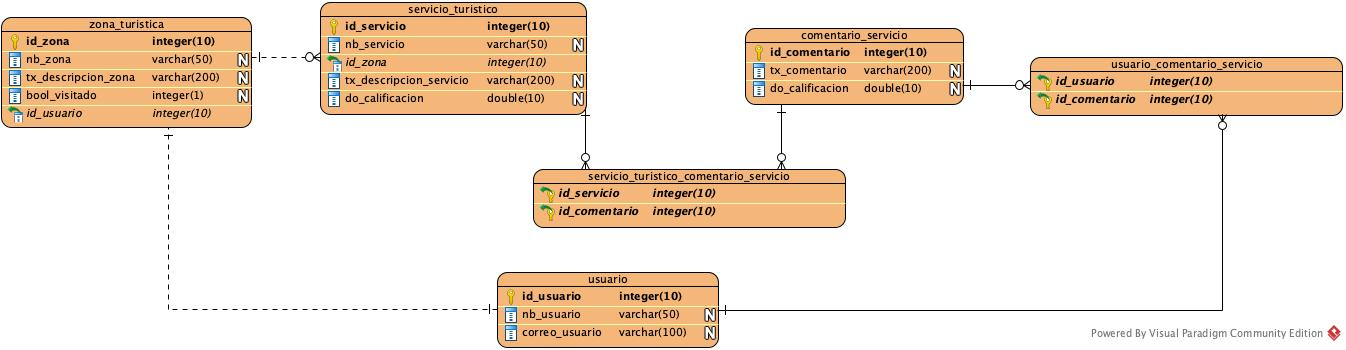
\includegraphics[angle=90, scale=.4]{casosDeUso/images/base_datos_v1.jpg}
				\caption{Base de datos}
			}
			\label{fig:base_datos_v1}
		\end{center}
	\end{figure}
}

\newpage
\section{Diagrama de clases}
Un diagrama de clases sirve para representar gráficamente la estructura de un sistema cuya implementación se llevará a cabo mediante un lenguaje de programación orientado a objetos. Dentro de la etapa de diseño y posterior al análisis de requerimientos es que se realiza el diagrama de clases para el sistema. El principal objetivo de estos diagramas es representar las clases y su contenido, así como su relación con otras clases \cite{clases}.

\subsection{Componentes de un diagrama de clases}
A continuación se describirán los componentes de un diagrama de clases, estos componentes se encuentran dentro del Lenguaje Unificado de Modelado (Unified Modeling Language, UML\footnote{\url{https://www.uml.org/}} por sus siglas en ingles)\footnote{De aquí en adelante se empleará UML para referirse al Lenguaje Unificado de Modelado}.

\begin{itemize}
	\item \textbf{Clase}: Es el componente básico para el diagrma de clases, estas representan las entidades o conceptos. Dentro de las clases se definen los atributos y métodos que utilizarán los objetos de la clase. La Figura \ref{fig:clase} muestra un ejemplo de como se representa una clase.
	
	\hypertarget{fig:clase}{
		\begin{figure}[htbp]
			\begin{center}
				\hypertarget{fig:clase}{
					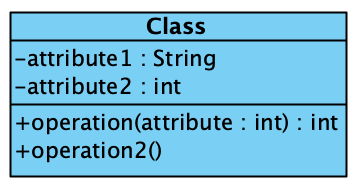
\includegraphics[ scale=.8]{analisisRequerimientos/clases/images/clase}
					\caption{Ejemplo de clase}
				}
				\label{fig:clase}
			\end{center}
		\end{figure}
	}

	\item \textbf{Atributos y métodos}: Los atributos generalmente se muestran sus nombres y con su tipo, mientras que los métodos además de su nombre se incluye su tipo de retorno, en caso de que tenga, y los parámetros de entrada que recibe. Así mismo, tanto atributos como métodos están acompañados de un símbolo antes de su nombre, estos símbolos representan:
	
	\begin{itemize}
		\item \textbf{+} representa atributos públicos.
		\item \textbf{-} representa atributos privados.
		\item \textbf{\#} representa atributos protegidos.
	\end{itemize}

	\item \textbf{Relaciones}: Ya que las clases se relacionan entre sí, existen distintos tipos de relaciones:
	
	\begin{itemize}
		\item \textbf{Generalización}: Representa una extensión o herencia de una clase de otra. La Figura \ref{fig:generalizacion} muestra un ejemplo de esta relación.
		
		\hypertarget{fig:generalizacion}{
			\begin{figure}[htbp]
				\begin{center}
					\hypertarget{fig:generalizacion}{
						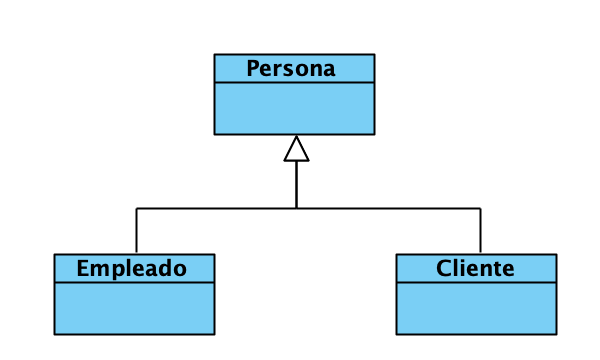
\includegraphics[ scale=.8]{analisisRequerimientos/clases/images/generalizacion}
						\caption{Ejemplo de generalizacion}
					}
					\label{fig:generalizacion}
				\end{center}
			\end{figure}
		}
		
		\newpage
		\item \textbf{Asociación}: Es una relación básica entre dos clases. Pueden ser unidireccionales (Figura \ref{fig:unidireccional}) o bidireccional (Figura \ref{fig:bidireccional}). 
		
		\hypertarget{fig:unidireccional}{
			\begin{figure}[htbp]
				\begin{center}
					\hypertarget{fig:unidireccional}{
						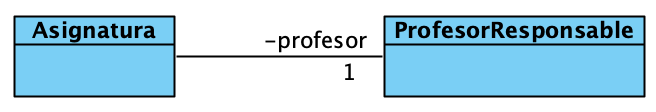
\includegraphics[ scale=.8]{analisisRequerimientos/clases/images/unidireccional}
						\caption{Ejemplo de unidireccional}
					}
					\label{fig:unidireccional}
				\end{center}
			\end{figure}
		}
		
		\hypertarget{fig:bidireccional}{
			\begin{figure}[htbp]
				\begin{center}
					\hypertarget{fig:bidireccional}{
						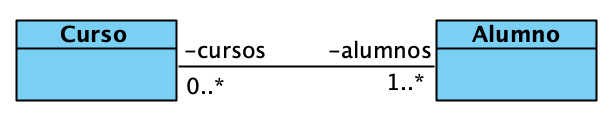
\includegraphics[ scale=.8]{analisisRequerimientos/clases/images/bidireccional}
						\caption{Ejemplo de bidireccional}
					}
					\label{fig:bidireccional}
				\end{center}
			\end{figure}
		}
	
		\item \textbf{Agregación}: Representa que un objeto de una clase contiene objetos de otra clase. La Figura \ref{fig:agragacion} muestra un ejemplo de una agregación.
		
		\hypertarget{fig:agragacion}{
			\begin{figure}[htbp]
				\begin{center}
					\hypertarget{fig:agragacion}{
						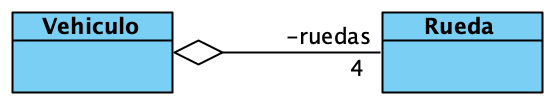
\includegraphics[ scale=.8]{analisisRequerimientos/clases/images/agregacion}
						\caption{Ejemplo de agragacion}
					}
					\label{fig:agragacion}
				\end{center}
			\end{figure}
		}
		
		\newpage
		\item \textbf{Composición}: Es una agregación fuerte, es decir, si un objeto contenido dentro de otra clase deja de existir no tiene sentido que el objeto contenedor siga existiendo. La Figura \ref{fig:composicion} muestra un ejemplo de una compisición.
		
			\hypertarget{fig:composicion}{
			\begin{figure}[htbp]
				\begin{center}
					\hypertarget{fig:composicion}{
						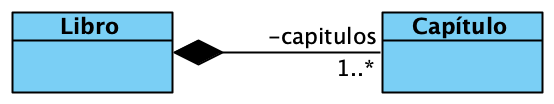
\includegraphics[ scale=.8]{analisisRequerimientos/clases/images/composicion}
						\caption{Ejemplo de composicion}
					}
					\label{fig:composicion}
				\end{center}
			\end{figure}
		}
		
	\end{itemize}
\end{itemize}

\subsection{Diagrama de clases del sistema}
La Figura \ref{fig:diagramaClases} muestra el diagrama de clases que fue definido para el desarrollo del proyecto.

\hypertarget{fig:diagramaClases}{
	\begin{figure}[htbp]
		\begin{center}
			\hypertarget{fig:diagramaClases}{
				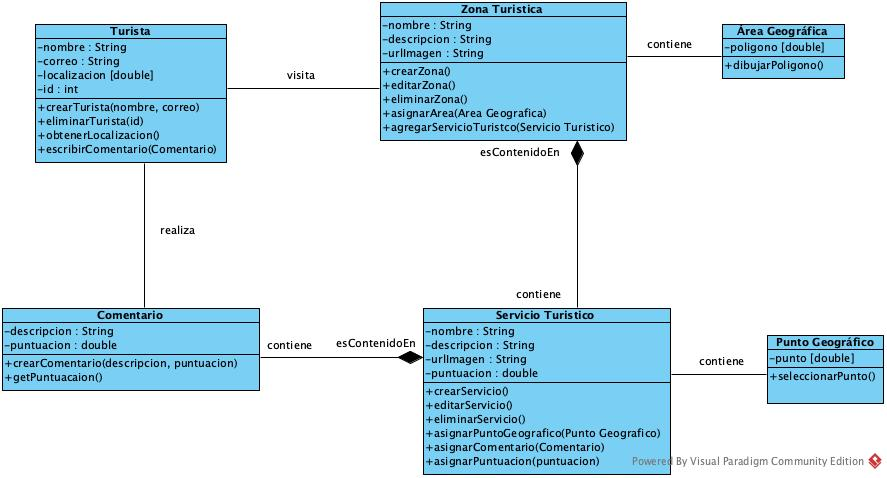
\includegraphics[ scale=.4]{analisisRequerimientos/clases/images/diagramaClases}
				\caption{Diagrama de clases del sistema}
			}
			\label{fig:diagramaClases}
		\end{center}
	\end{figure}
}
\newpage
\section{Diagramas de Secuencia}
El diagrama de secuencia es el encargado de mostrar la interacción que tiene un conjunto de objetos pertenecientes a una apliación en un cierto lapso de tiempo, en el cual se indican los módulos o clases que forman parte del sistema y las llamadas entre ellos para realizar una tarea específica. Estos diagramas permiten observar la perspectiva cronológica de las interacciónes que tiene el sistema \cite{secuencia}

\subsection{Diagrama de secuencia del sistema}
La Figura \ref{fig:diagramaSecuencia} muestra el diagrama de secuencia del sistema.

\hypertarget{fig:diagramaSecuencia}{
	\begin{figure}[htbp]
		\begin{center}
			\hypertarget{fig:diagramaSecuencia}{
				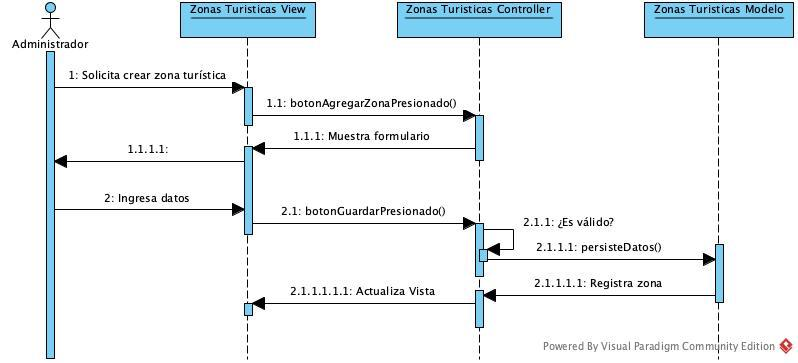
\includegraphics[ scale=.4]{analisisRequerimientos/secuencia/images/diagramaSecuencia}
				\caption{Diagrama de secuencia del sistema}
			}
			\label{fig:diagramaSecuencia}
		\end{center}
	\end{figure}
}

\newpage
\section{Análisis de casos de uso}
Para el análisis de casos de uso se tomaron en cuenta los requerimientos funcionales y los no funcionales, descritos en la sección anterior, que fueron identificados a partir de la propuesta de solución. \\

Para poder llevar a cabo un correcto análisis de casos de uso primero se tuvo que tener bien identificados a loa actores o usuarios finales que participarán en el uso del sistema. Una vez identificados se realizó una arquitectura de solución en la cual se definieron los módulos a desarrollar para el sistema, el análisis de casos de uso parte tomando como base estos módulos ya que en ellos será donde se centre la interacción del usuario con el sistema. \\

En la Figura \ref{fig:casosDeUso} se muestra el diagrama general de los casos de uso identificados para el sistema, en él puede observarse que los casos de uso se encuentran divididos por paquetes que corresponden a las aplicaciones que conforman el sistema, y que cada uno de estos tiene un nombre.


\hypertarget{fig:casosDeUso}{
	\begin{figure}[htbp]
		\begin{center}
			\hypertarget{fig:casosDeUso}{
				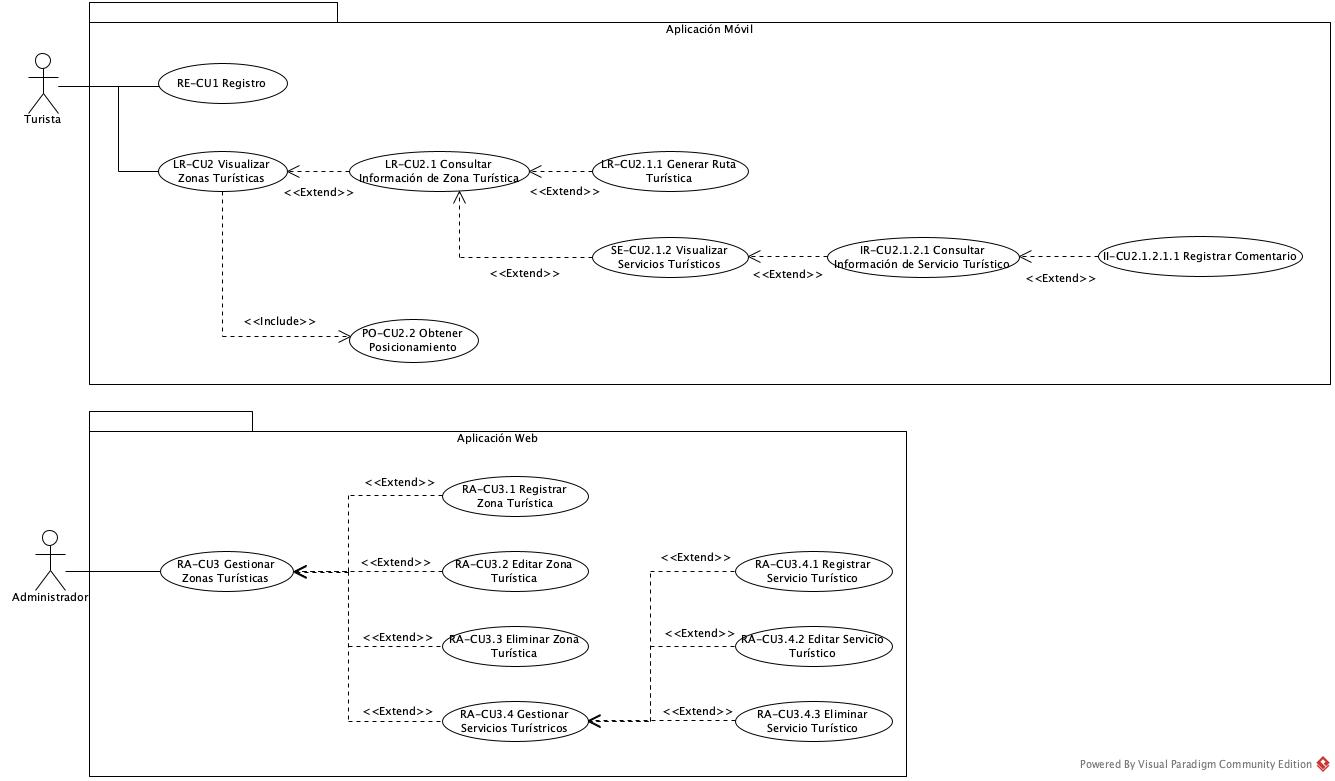
\includegraphics[angle=90, scale=.4]{casosDeUso/images/DiagramaDeCasosDeUso}
				\caption{Diagrama de casos de uso}
			}
			\label{fig:casosDeUso}
		\end{center}
	\end{figure}
}

\newpage
A continuación se muestra la nomenclatura utilizada para asignar el nombre a los casos de uso:

\begin{center}
	\Huge{\textit{Iniciales\_módulo}-CU\textit{n}: \textit{nombre\_caso\_de\_uso}}
\end{center}

Donde: 

\begin{itemize}
	\item \textbf{iniciales\_módulo}: significa que son las iniciales del módulo en el que se encuentra el caso de uso, los módulos son: 
	\begin{itemize}
		\item RE: Registro
		\item LR: Localización de rutas
		\item PO: Posicionamiento
		\item II: Interacción de la información
		\item SE: Servicios
		\item IR: Información y representación de estadísticas turísticas
		\item RA: Registro de área turística
	\end{itemize}

	\item \textbf{n}: es el número de caso de uso.
	
	\item \textbf{nombre\_caso\_de\_uso}: es el nombre del caso de uso.
\end{itemize}

Para realizar la documentación se tomaron los casos de uso y se separaron por módulo. Cabe mencionar que aunque sean distintos módulos los casos de uso tienen una relación entre sí para poder construir el sistema. \\

La documentación de los casos de uso se divide en tres partes:

\begin{enumerate}
	\item Descripción
	\item Atributos
	\item Trayectorias
\end{enumerate}

La descripción es un breve resumen de lo que trata el caso de uso, en ella se describe el por qué del caso de uso, para qué es importante tenerlo, el objetivo principal y lo que se obtiene al ejecutarlo.\\

Los atributos son descritos en una tabla, esto facilita al desarrollador identificar las entradas y salidas del caso de uso, su precedencia y los cambios que produce al sistema. \\

La trayectoria son los pasos a seguir para la correcta ejecución y desarrollo del caso de uso, en esta puede haber trayectorias alternativas, puntos de extensión a otros casos de uso o inclusión de otros casos casos de uso. \\

Las tablas \cdtRef{RE-CU1}{3.7.2} a la \cdtRef{RE-CU3.4.3}{2.23.2} muestran los atributos más importantes del caso de uso al cual pertenecen.

A continuación se detallan los casos de uso:

<<<<<<< HEAD

% !TeX spellcheck = <none>
% \IUref{IUAdmPS}{Administrar Planta de Selección}
% \IUref{IUModPS}{Modificar Planta de Selección}
% \IUref{IUEliPS}{Eliminar Planta de Selección}

% 


% Copie este bloque por cada caso de uso:
%-------------------------------------- COMIENZA descripción del caso de uso.

%\begin{UseCase}[archivo de imágen]{UCX}{Nombre del Caso de uso}{
%--------------------------------------
	\begin{UseCase}{CU6}{Registrar Comentario}{
		Este caso de uso permite al usuario registrar un comentario y una puntuación a un servicio turístico seleccionado que se encuentre dentro de un área registrada. Cabe destacar que para poder acceder a este caso de uso es necesario que se valide la regla de negocio XXXXX .
	}
		\UCitem{Versión}{\color{Gray}1.0}
		\UCitem{Actor}{\hyperlink{Usuario}{Usuario}}
		\UCitem{Propósito}{Registrar un comentario y puntuación.}
		\UCitem{Entradas}{Comentario y Puntuación}
		\UCitem{Origen}{Teclado}
		\UCitem{Salidas}{N.A.}
		\UCitem{Precondiciones}{Cumplir con la regla de negocio XXXXXX}
		\UCitem{Postcondiciones}{Quedará el comentario y la puntuación, asociada al servicio turístico}
		\UCitem{Errores}{}
		\UCitem{Tipo}{Caso de uso Cuaternario}
		\UCitem{Observaciones}{}
	\end{UseCase}
%--------------------------------------
	\begin{UCtrayectoria} 
		
		\UCpaso[\UCactor] Da clic en el botón \IUbutton{Comentar} de la pantalla  \IUref{IU8}{Principal}.
		
		\UCpaso Obtiene la descripción, puntuación y los comentarios del servicio seleccionado.
		
		\UCpaso Verifica que el usuario tenga permitido comentar mediante la regla de negocio XXXXXXXXXX. \Trayref{A}.
		
		\UCpaso Despliega la pantalla \IUref{IU8}{Principal} con los datos asociados al servicio, así como habilitados los botones \IUbutton{Ver Mapa} y \IUbutton{Comentar}.
		
		\UCpaso[] Termina el caso de uso.
		
	\end{UCtrayectoria}

%--------------------------------------		
		\begin{UCtrayectoriaA}{A}{El usuario no tiene permitido realizar un comentario.}
			
		\UCpaso Despliega la pantalla \IUref{IU8}{Principal} con los datos asociados al servicio y únicamente habilitado el botón \IUbutton{Ver Mapa}.
		
		\UCpaso[] Termina el caso de uso.
		
	\end{UCtrayectoriaA}
	
	
=======
% !TeX spellcheck = <none>
% \IUref{IUAdmPS}{Administrar Planta de Selección}
% \IUref{IUModPS}{Modificar Planta de Selección}
% \IUref{IUEliPS}{Eliminar Planta de Selección}

% 


% Copie este bloque por cada caso de uso:
%-------------------------------------- COMIENZA descripción del caso de uso.

%\begin{UseCase}[archivo de imágen]{UCX}{Nombre del Caso de uso}{
%--------------------------------------
	\begin{UseCase}{CU6}{Registrar Comentario}{
		Este caso de uso permite al usuario registrar un comentario y una puntuación a un servicio turístico seleccionado que se encuentre dentro de un área registrada. Cabe destacar que para poder acceder a este caso de uso es necesario que se valide la regla de negocio XXXXX .
	}
		\UCitem{Versión}{\color{Gray}1.0}
		\UCitem{Actor}{\hyperlink{Usuario}{Usuario}}
		\UCitem{Propósito}{Registrar un comentario y puntuación.}
		\UCitem{Entradas}{Comentario y Puntuación}
		\UCitem{Origen}{Teclado}
		\UCitem{Salidas}{N.A.}
		\UCitem{Precondiciones}{Cumplir con la regla de negocio XXXXXX}
		\UCitem{Postcondiciones}{Quedará el comentario y la puntuación, asociada al servicio turístico}
		\UCitem{Errores}{}
		\UCitem{Tipo}{Caso de uso Cuaternario}
		\UCitem{Observaciones}{}
	\end{UseCase}
%--------------------------------------
	\begin{UCtrayectoria} 
		
		\UCpaso[\UCactor] Da clic en el botón \IUbutton{Comentar} de la pantalla  \IUref{IU8}{Principal}.
		
		\UCpaso Obtiene la descripción, puntuación y los comentarios del servicio seleccionado.
		
		\UCpaso Verifica que el usuario tenga permitido comentar mediante la regla de negocio XXXXXXXXXX. \Trayref{A}.
		
		\UCpaso Despliega la pantalla \IUref{IU8}{Principal} con los datos asociados al servicio, así como habilitados los botones \IUbutton{Ver Mapa} y \IUbutton{Comentar}.
		
		\UCpaso[] Termina el caso de uso.
		
	\end{UCtrayectoria}

%--------------------------------------		
		\begin{UCtrayectoriaA}{A}{El usuario no tiene permitido realizar un comentario.}
			
		\UCpaso Despliega la pantalla \IUref{IU8}{Principal} con los datos asociados al servicio y únicamente habilitado el botón \IUbutton{Ver Mapa}.
		
		\UCpaso[] Termina el caso de uso.
		
	\end{UCtrayectoriaA}
	
	
% !TeX spellcheck = <none>
% \IUref{IUAdmPS}{Administrar Planta de Selección}
% \IUref{IUModPS}{Modificar Planta de Selección}
% \IUref{IUEliPS}{Eliminar Planta de Selección}

% 


% Copie este bloque por cada caso de uso:
%-------------------------------------- COMIENZA descripción del caso de uso.

%\begin{UseCase}[archivo de imágen]{UCX}{Nombre del Caso de uso}{
%--------------------------------------
	\begin{UseCase}{CU6}{Registrar Comentario}{
		Este caso de uso permite al usuario registrar un comentario y una puntuación a un servicio turístico seleccionado que se encuentre dentro de un área registrada. Cabe destacar que para poder acceder a este caso de uso es necesario que se valide la regla de negocio XXXXX .
	}
		\UCitem{Versión}{\color{Gray}1.0}
		\UCitem{Actor}{\hyperlink{Usuario}{Usuario}}
		\UCitem{Propósito}{Registrar un comentario y puntuación.}
		\UCitem{Entradas}{Comentario y Puntuación}
		\UCitem{Origen}{Teclado}
		\UCitem{Salidas}{N.A.}
		\UCitem{Precondiciones}{Cumplir con la regla de negocio XXXXXX}
		\UCitem{Postcondiciones}{Quedará el comentario y la puntuación, asociada al servicio turístico}
		\UCitem{Errores}{}
		\UCitem{Tipo}{Caso de uso Cuaternario}
		\UCitem{Observaciones}{}
	\end{UseCase}
%--------------------------------------
	\begin{UCtrayectoria} 
		
		\UCpaso[\UCactor] Da clic en el botón \IUbutton{Comentar} de la pantalla  \IUref{IU8}{Principal}.
		
		\UCpaso Obtiene la descripción, puntuación y los comentarios del servicio seleccionado.
		
		\UCpaso Verifica que el usuario tenga permitido comentar mediante la regla de negocio XXXXXXXXXX. \Trayref{A}.
		
		\UCpaso Despliega la pantalla \IUref{IU8}{Principal} con los datos asociados al servicio, así como habilitados los botones \IUbutton{Ver Mapa} y \IUbutton{Comentar}.
		
		\UCpaso[] Termina el caso de uso.
		
	\end{UCtrayectoria}

%--------------------------------------		
		\begin{UCtrayectoriaA}{A}{El usuario no tiene permitido realizar un comentario.}
			
		\UCpaso Despliega la pantalla \IUref{IU8}{Principal} con los datos asociados al servicio y únicamente habilitado el botón \IUbutton{Ver Mapa}.
		
		\UCpaso[] Termina el caso de uso.
		
	\end{UCtrayectoriaA}
	
	
>>>>>>> 4b243b0421e3340fd688e8e3a78460d652bbf8cd



%=========================================================
%%=========================================================
\chapter{Modelo del Alcance}
\label{cap:reqUsr}

	En este capítulo se modela el alcance del sistema. Se presentan inicialmente los Actores involucrados y sus requerimientos, especificando cuales se alcanzaron en la primera iteración y cuales serán trabajados en la segunda iteración. Después se presentan los requerimientos funcionales de esta iteración y al final se presenta el modelo Físico y Lógico del sistema.


%---------------------------------------------------------
\section{Modelado de Usuarios}
\cdtInstrucciones{
	Identifique los actores que estarán involucrados en los procesos relacionados con el sistema para esta iteración de desarrollo. Ponga énfasis en los procesos involucrados.
}

\subsection{Organigrama de la Empresa}

	

\begin{figure}[htbp]
	\begin{center}
		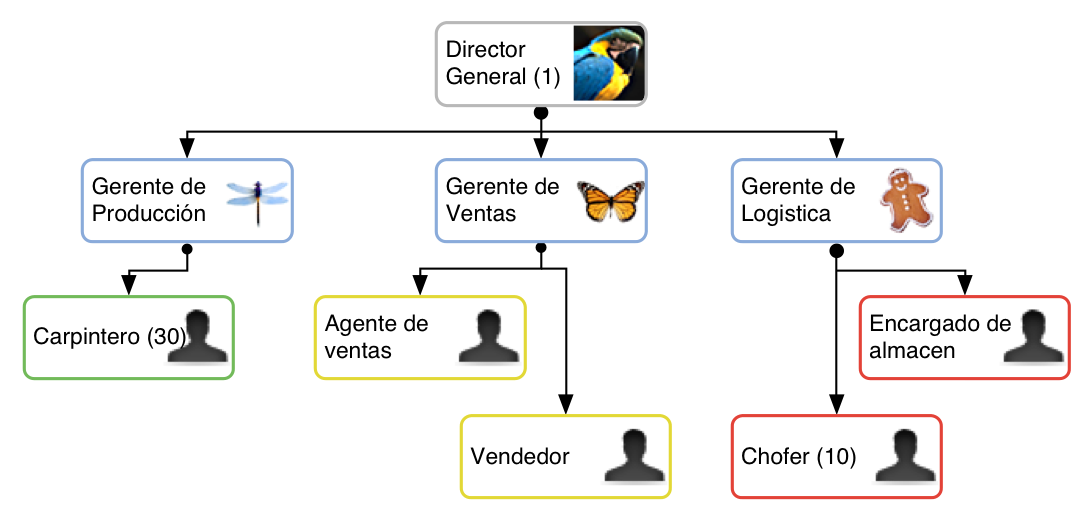
\includegraphics[width=.8\textwidth]{images/organigramaEm}
		\caption{Organigrama de la Mueblería Qetzal S. A. de C. V.}
		\label{fig:organigrama}
	\end{center}
\end{figure}


%---------------------------------------------------------
\begin{Usuario}{\subsection{Gerente de Ventas}}{
	Es el encargado de todas las operaciones de ventas al mayoreo y al menudeo. coordina y supervisa el trabajo de los Agentes de Ventas y Encargados de Tienda.
	Reporta directamente al Gerente de Operaciones
}
    \item[Responsabilidades:] \cdtEmpty
    \begin{itemize}
		\item Supervisar la operación de ventas.
		\item Plantear y supervisar el logro de las metas de ventas de la empresa y su crecimiento económico.
		\item ...
    \end{itemize}

	\item[Perfil:] \cdtEmpty
    \begin{itemize}
		\item Amplia experiencia en el ramo.
		\item Licenciatura como mínimo.
		\item ...
    \end{itemize}
	\item[Procesos en los que participa:] \cdtEmpty
    \begin{itemize}
		\item PC-V01 Aprobar las ordenes de compra al mayoreo.
		\item PC-V02 Supervisar las ventas al menudeo.
		\item PC-V03 Elaborar informe de ventas mensual.
		\item ...
    \end{itemize}
\end{Usuario}

%---------------------------------------------------------
\begin{Usuario}{\subsection{Agente de Ventas}}{
	...
}
    \item[Responsabilidades:] \cdtEmpty
    \begin{itemize}
		\item ...
    \end{itemize}

	\item[Perfil:] \cdtEmpty
    \begin{itemize}
		\item ...
    \end{itemize}
	\item[Procesos en los que participa:] \cdtEmpty
    \begin{itemize}
		\item PC-V08 Venta al Mayoreo.
		\item ...
    \end{itemize}
\end{Usuario}


%---------------------------------------------------------
\section{Requerimientos de usuario}

\cdtInstrucciones{
	Identifique y describa los requerimientos funcionales del sistema señalando: id, nombre, descripción y prioridad.
}

\begin{table}[htbp!]
	\begin{requerimientosU}
		\FRitem{RU1}{Control de vehículos}{El usuario requiere llevar un registro actualizado de los vehículos, sus características y su estado.}{1}{\DONE}
		\FRitem{RU2}{Registro de ventas}{El usuario requiere llevar un registro actualizado de todas las ventas realizadas por mes y su status: pedido, entregado, pagado, etc..}{2}{\TODO}
		\FRitem{RU3}{Registro de clientes}{El usuario requiere llevar un registro actualizado de todos los clientes para su seguimiento, atención y tareas de promoción y mercadotecnia.}{1}{\DONE}
		\FRitem{RU4}{Planeación de entregas}{El usuario requiere una herramienta que le facilite la planeación de vehículos para que esta sea la más adecuada.}{-}{\DOING}
		\FRitem{...}{...}{...}{...}{...}
	\end{requerimientosU}
    \caption{Requerimientos funcionales del sistema.}
    {\footnotesize\em Para leer correctamente esta tabla vea la leyenda en la Tabla~\ref{tbl:leyendaRF} en la página~\pageref{tbl:leyendaRF}.}
    \label{tbl:reqFunc}
\end{table}



%---------------------------------------------------------
\section{Especificación de plataforma}	

\cdtInstrucciones{
	Coloque un diagrama y su descripción para aclarar el tipo de solución propuesta. \\
	
 En esta sección se debe aclarar:
	
\begin{description}
	\item[Tipo de sistema:] Web, aplicación móvil, de escritorio, híbrida, etc.
	\item[Software requerido:] Programas que se deberán instalar, desde el sistema operativo, compiladores, interpretes, servidores, etc.
	\item[Hardware requerido:] CPU, núcleos, velocidad, memoria, disco duro, etc.
	\item[servicios:] De conexión, seguridad, firewall, respaldo de energía, redundancia, uso de raids, etc.
\end{description}
}

\begin{figure}[htbp!]
	\begin{center}
		\fbox{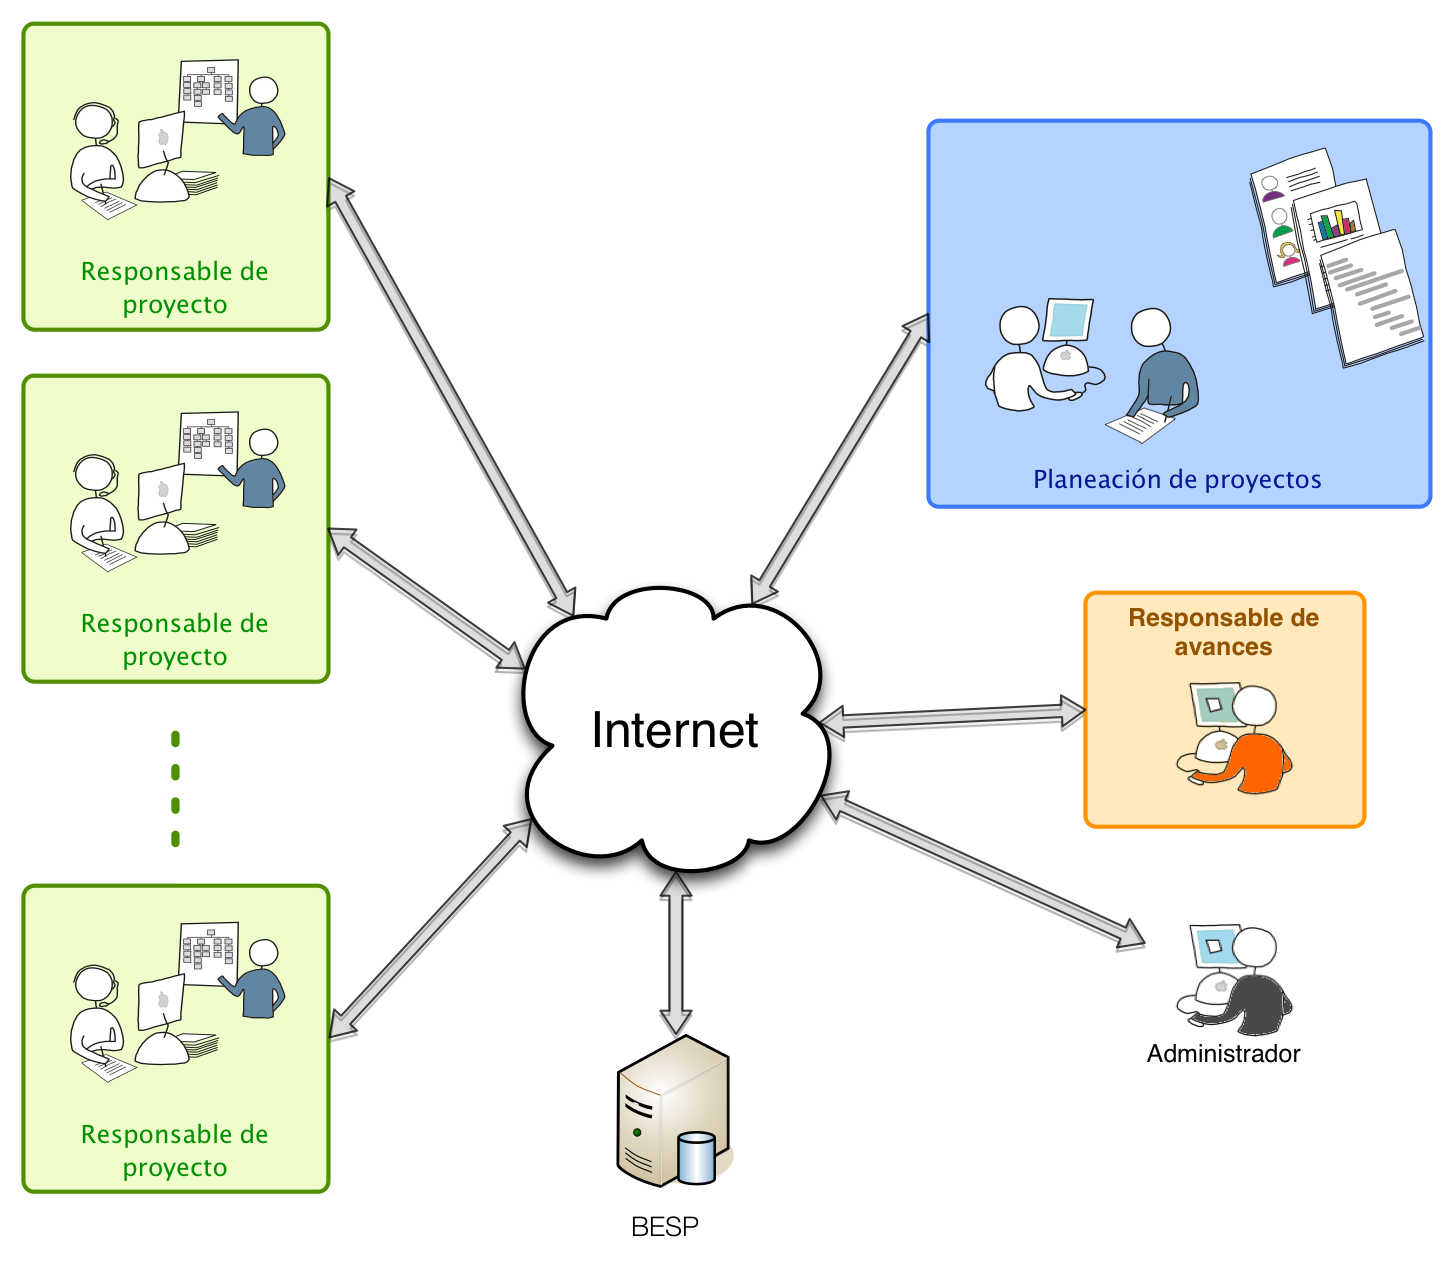
\includegraphics[width=.6\textwidth]{images/arquitectura}}
		\caption{Arquitectura del sistema.}
		\label{fig:arquitectura}
	\end{center}
\end{figure}

En la figura~\ref{fig:arquitectura} se describe la estructura del sistema, en ella se detalla ...



%
%%=========================================================
%%=========================================================
\chapter{Modelo del Negocio}	
\label{cap:reqSist}

	En este capítulo se modela la {\em Arquitectura del negocio} la cual está conformada por la Ontología del negocio ({\em Términos} y {\em Hechos del negocio}), Arquitectura de procesos y las {\em Reglas del negocio}. Primero se especifica brevemente el {\em Contexto} en el que los términos tienen significado.
	
	En las secciones \ref{sec:terminosDeNegocio} y \ref{sec:hechosDeNegocio} se presentan los Términos del negocio a manera de Glosario y por último se presentan los Hechos del negocio a manera de relaciones entre términos del negocio.

%----------------------------------------------------------
\section{Contexto}

	\cdtInstrucciones{El contexto debe explicar bajo que ambiente los términos del negocio son aplicables y proporcionar información general para su comprensión inicial.\\}
	La empresa ``Fast Rent'' se dedica a la renta de vehículos automotores, principalmente automóviles y motocicletas. Los clientes rentan vehículos por tiempos determinados y la empresa se encarga de dar mantenimiento a los vehículos y administrarlos para que estén disponibles para sus clientes. Los empleados, se dedican a labores de gerencia, atención a clientes, mantenimiento y soporte para los vehículos activos.
	
%---------------------------------------------------------
\section{Términos del Negocio}
\label{sec:terminosDeNegocio}

\begin{description}
	% Ejemplo de un término literal.
	\item[\hypertarget{tAutomovil}{Automóvil:}] ({\em es un tipo de \hyperlink{tVehiculo}{Vehículo}}) De cuatro ruedas con capacidad de 5 a 9 personas. 
	% Ejemplo de un término de entidad
	\item[\hypertarget{tCliente}{Cliente:}] Se refiere a todas las personas físicas y morales que \hyperlink{tRenta}{rentan} o han rentado un \hyperlink{tVehiculo}{vehículo}.
	
	\item[\hypertarget{tDirector}{Director:}] ({\em es un tipo de \hyperlink{tEmpleado}{Empleado}}) Es el empleado que tiene mayor rango de todos y no tiene superior, a diferencia de los demás.	
	\item[\hypertarget{tEmpleado}{Empleado:}] Se refiere a cualquier persona que labore en la empresa.
	
	\item[\hypertarget{tChecador}{Checador:}] ({\em Reloj asociado al atributo:} Hora de entrada y salida de un \hyperlink{tEmpleado}{empleado}. {\em Frecuencia de lectura:} Una vez al día para la entrada y otra para la salida durante los días laborales.
	
	\item[\hypertarget{tMotocicleta}{Motocicleta:}] ({\em es un tipo de {tVehiculo}{Vehículo}}) De dos ruedas con capacidad para una personas. 

	\item[\hypertarget{tRenta}{Renta:}] Se refiere al servicio que ofrece la empresa para prestar \hyperlink{tVehiculo}{vehículos} a los \hyperlink{tCliente}{clientes} por un tiempo definido.
	
	\item[\hypertarget{tVehiculo}{Vehiculo:}] Se refiere a los automóviles y motocicletas que la empresa usa para dar el servicio de renta a los \hyperlink{tCliente}{clientes}.
	
%	\brTermSensor{tVelocimetro}{Velocímetro:}{Velocidad de un Vehículo.}{Kilometros/hora.}{Constantemente siempre que el \cdtRef{tVehiculo}{vehículo} esté encendido.}
\end{description}

%----------------------------------------------------------
\section{Modelo del dominio del problema}
\label{sec:hechosDeNegocio}


%- - - - - - - - - - - - - - - - - - - - - - - - - - - - - 
\subsection{Modelo del dominio del problema}

	El modelo del dominio del problema se muestra en la figura~\ref{fig:modeloDeDominio}, a continuación se describen cada una de las entidades y sus relaciones.
	
\begin{figure}[htbp!]
	\begin{center}
		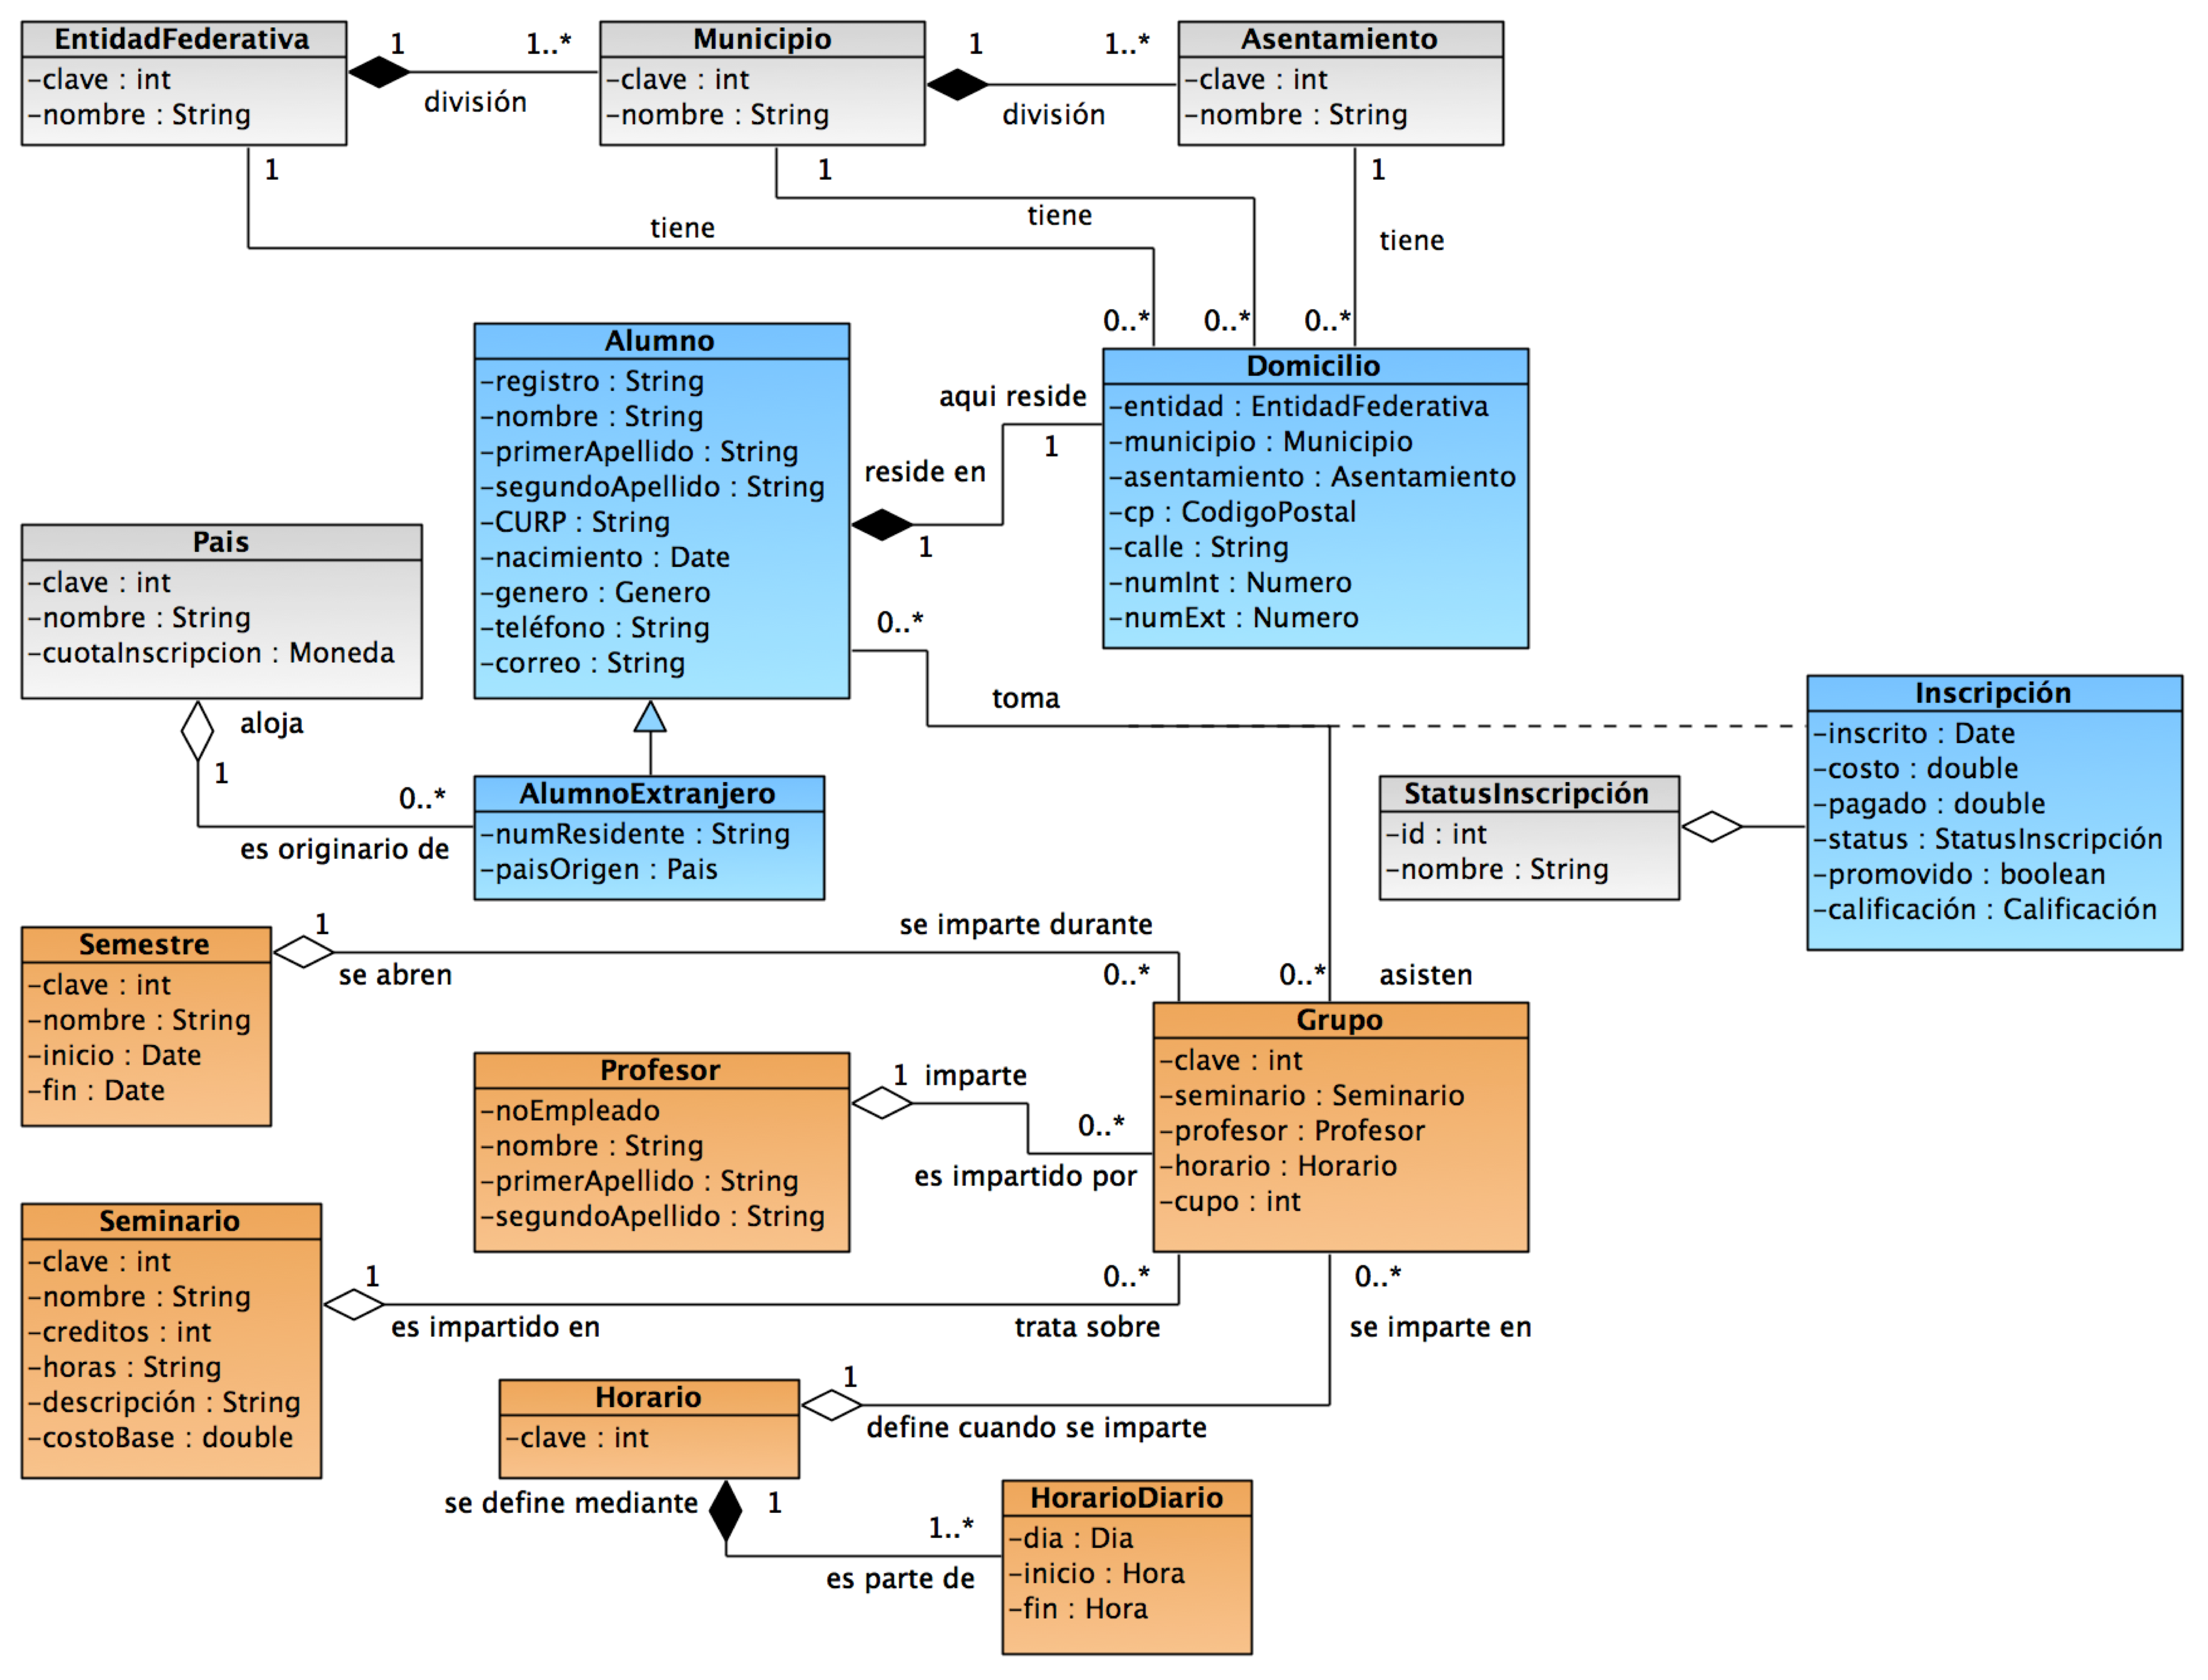
\includegraphics[angle=90,width=.95\textwidth]{images/modeloDelDominioDelProblema}
		\caption{Modelo del dominio del problema}
		\label{fig:modeloDeDominio}
	\end{center}
\end{figure}

\begin{cdtEntidad}{Alumno}{Alumno}
	\brAttr{registro}{Registro}{Id}{Número de registro utilizado para identificar un alumno}{Sí}
	\brAttr{nombre}{Nombre}{Palabra Corta}
		{Nombre o nombres del alumno.}{Sí}
	\brAttr{primerApellido}{Primer apellido}{Palabra Corta}
		{Primer apellido del alumno.}{Sí}
	\brAttr{segundoApellido}{Segundo apellido}{Palabra Corta}
		{Segundo apellido del alumno.}{No}
	\brAttr{CURP}{CURP}{CURP}
		{CURP del alumno.}{Sí}
	\brAttr{nacimiento}{Nacimiento}{Fecha}
		{Fecha de nacimiento del alumno.}{Sí}
	\brAttr{genero}{Género}{Domicilio}
		{Género del alumno.}{No}
	\brAttr{telefono}{Teléfono}{Telefono}
		{Teléfono para contactar al alumno.}{Sí}
	\brAttr{correo}{Correo}{Correo}
		{Correo del alumno para enviar información académica y escolar y para recuperación de clave de acceso.}{Sí}
	\cdtEntityRelSection
	\brRel{\brRelComposition}{Domicilio}{Un \hyperlink{Alumno}{Alumno} reside en un \hyperlink{Domicilio}{Domicilio}}	
	\brRel{\brRelAgregation}{Grupo}{Un \hyperlink{Alumno}{Alumno} toma un \hyperlink{Curso}{Curso}}	
\end{cdtEntidad}

%- - - - - - - - - - - - - - - - - - - - - - - - - - - - - 
\begin{cdtEntidad}{AlumnoExtranjero}{Alumno Extranjero}%{}
	\brAttr{numeroResidente}{Numero de residente}{Id}{Número de registro dado por la Secretaría de Relaciones Exteriores a los extranjeros.}{Si}
	\brAttr{paisOrigen}{Pais origen}{\hyperlink{Pais}{País}}
		{País de origen del alumno extranjero.}{Sí}
	\cdtEntityRelSection
	\brRel{\brRelAgregation}{País}{Un \hyperlink{Alumno}{Alumno} es originario de un \hyperlink{Pais}{Pais}}	
	\brRel{\brRelGeneralization}{Alumno}{Un \hyperlink{AlumnoExtranjero}{Alumno Extranjero} es un  \hyperlink{Alumno}{Alumno}}	
\end{cdtEntidad}

%---------------------------------------------------------
\section{Modelado de Reglas de negocio}

\begin{BussinesRule}{BR8}{Fecha de Nacimiento correcta.}
	\BRitem[Tipo:] Regla de integridad referencial o estructural. 
				% Otras opciones para tipo: 
				% - Regla de integridad referencial o estructural. 
				% - Regla de operación, (calcular o determinar un valor.).
				% - Regla de inferencia de un hecho.
	\BRitem[Clase:] Habilitadora. 
				% Otras opciones para clase: Habilitadora, Cronometrada, Ejecutive.
	\BRitem[Nivel:] Control. % Otras opciones para nivel: Control, Influencia.
	\BRitem[Descripción:]	Las Fechas de Nacimiento que se registran en el SINACEM para cualquier Persona debe ser mayores al día Primero de Enero del año 1900 y menor a la Fecha Actual.
	\BRitem[Motivación:] Evitar fraudes al PRONIM por el registro de personas que no han nacido al momento de su registro.
	\BRitem[Sentencia:] $\forall p \in Persona \Rightarrow 01-Enero-1900~<~p.fechaDeNacimiento~<~fechaActual$.
	\BRitem[Ejemplo positivo:] Para el día 12 de Octubre del 2013, cumplen la regla: 		
        \begin{itemize}
        	\item 11 de Octubre del 2013
			\item 20 de Diciembre del 2010
			\item 2 de Enero del 1900
        \end{itemize}
	
	\BRitem[Ejemplo negativo:] Para el día 12 de Octubre del 2013, no cumplen la 
		\begin{itemize}
        	\item 12 de Octubre del 2013
			\item 20 de Diciembre del 2014
			\item 1 de Enero del 1900
			\item 31 de Diciembre del 1899
        \end{itemize}
	
	\BRitem[Referenciado por:] \hyperlink{CUCE3.2}{CUCE3.2}, \hyperlink{CUCE3.3}{CUCE3.3}.
\end{BussinesRule}

\begin{BussinesRule}{BR129}{Determinar si un Estudiante puede inscribir Seminario.} 
	\BRitem[Tipo:] Regla de integridad referencial o estructural. 
				% Otras opciones para tipo: 
				% - Regla de integridad referencial o estructural. 
				% - Regla de operación, (calcular o determinar un valor.).
				% - Regla de inferencia de un hecho.
	\BRitem[Clase:] Habilitadora. 
				% Otras opciones para clase: Habilitadora, Cronometrada, Ejecutive.
	\BRitem[Nivel:] Control. % Otras opciones para nivel: Control, Influencia.
	\BRitem[Descripción:] Un Estudiante requere del 80\% de créditos para inscribirse a un Seminario y no haber cursado y reprobado otro seminario.
	\BRitem[Ejemplo positivo:] 
	
	\BRitem[Ejemplo negativo:] 
	
	\BRitem[Referenciado por:] 
\end{BussinesRule}

\begin{BussinesRule}{BR130}{Determinar si un Estudiante puede inscribirse en un Seminario}
	\BRitem[Tipo:] Regla de inferencia de un hecho.
				% Otras opciones para tipo: 
				% - Regla de integridad referencial o estructural. 
				% - Regla de operación, (calcular o determinar un valor.).
				% - Regla de inferencia de un hecho.
	\BRitem[Clase:] Habilitadora. 
				% Otras opciones para clase: Habilitadora, Cronometrada, Ejecutive.
	\BRitem[Nivel:] Control. % Otras opciones para nivel: Control, Influencia.
	\BRitem[Descripción:] El Estudiante debe pertenecer a la Carrera del Seminario y debe haber Cupo en el grupo del Seminario.
	\BRitem[Ejemplo positivo:] 
	
	\BRitem[Ejemplo negativo:] 
	
	\BRitem[Referenciado por:] 
\end{BussinesRule}

\begin{BussinesRule}{BR143}{Validar el horario del estudiante}
	\BRitem[Tipo:] Regla de operación, (calcular o determinar un valor.).
				% Otras opciones para tipo: 
				% - Regla de integridad referencial o estructural. 
				% - Regla de operación, (calcular o determinar un valor.).
				% - Regla de inferencia de un hecho.
	\BRitem[Clase:] Habilitadora. 
				% Otras opciones para clase: Habilitadora, Cronometrada, Ejecutive.
	\BRitem[Nivel:] Control. % Otras opciones para nivel: Control, Influencia.
	\BRitem[Descripción:] Las Materias y Seminarios inscritos por el alumno, en un periodo específico, no pueden impartirse en el mismo día de la semana en horas traslapadas.
	\BRitem[Ejemplo positivo:] 
	
	\BRitem[Ejemplo negativo:] 
	
	\BRitem[Referenciado por:] 
\end{BussinesRule}

\begin{BussinesRule}{BR180}{Calcular costos del Estudiante}
	\BRitem[Tipo:] Regla de operación, (calcular o determinar un valor.).
				% Otras opciones para tipo: 
				% - Regla de integridad referencial o estructural. 
				% - Regla de operación, (calcular o determinar un valor.).
				% - Regla de inferencia de un hecho.
	\BRitem[Clase:] Habilitadora. 
				% Otras opciones para clase: Habilitadora, Cronometrada, Ejecutive.
	\BRitem[Nivel:] Control. % Otras opciones para nivel: Control, Influencia.
	\BRitem[Descripción:] Los servicios se cobran de la siguiente forma:
		\begin{Citemize}
			\item {\em Estudiantes Regulares:} Se les Cobran todos los servicios al 100\% de su costo.
			\item {\em Estudiantes becados:} Se les otorga un 80\% de descuento en el costo de todos los servicios (antes del IVA).
			\item {\em Estudiantes extranjeros:} Se les cobran los servicios al 200\% del costo registrado.
		\end{Citemize}
	\BRitem[Sentencia:] $\forall~e~\in~\mathbb{E}\textrm{studiantes}~\land~\forall~s~\in \mathbb{S}\textrm{eminario}~\Rightarrow$
		\begin{displaymath}
			Costo(e,s) = \left\{ \begin{array}{ll}
			s.costo & , si~e.tipo = \textrm{Estudiante regular}\\
			{s.costo}\over{5} & , si~e.tipo = \textrm{Estudiante becado}\\
			s.costo \cdot 2 & , si~e.tipo = \textrm{Estudiante extranjero}
			\end{array} \right.
		\end{displaymath}
	\BRitem[Ejemplo positivo:] 
	
	\BRitem[Ejemplo negativo:] 
	
	\BRitem[Referenciado por:] 
\end{BussinesRule}

\begin{BussinesRule}{BR45}{Calcular impuestos por seminario}
	\BRitem[Tipo:] Regla de operación, (calcular o determinar un valor.).
				% Otras opciones para tipo: 
				% - Regla de integridad referencial o estructural. 
				% - Regla de operación, (calcular o determinar un valor.).
				% - Regla de inferencia de un hecho.
	\BRitem[Clase:] Habilitadora. 
				% Otras opciones para clase: Habilitadora, Cronometrada, Ejecutive.
	\BRitem[Nivel:] Control. % Otras opciones para nivel: Control, Influencia.
	\BRitem[Descripción:] Los impuestos corresponden al 16\% correspondientes al IVA.
	\BRitem[Sentencia:] $Impuesto(e, s) = Costo(e, s)\cdot0.16$.
	\BRitem[Ejemplo positivo:] 
	
	\BRitem[Ejemplo negativo:] 
	
	\BRitem[Referenciado por:] 
\end{BussinesRule}

\begin{BussinesRule}{BR100}{Recibo del Estudiante por inscripción a Seminario.}
	\BRitem[Tipo:] Regla de operación, (calcular o determinar un valor.).
				% Otras opciones para tipo: 
				% - Regla de integridad referencial o estructural. 
				% - Regla de operación, (calcular o determinar un valor.).
				% - Regla de inferencia de un hecho.
	\BRitem[Clase:] Habilitadora. 
				% Otras opciones para clase: Habilitadora, Cronometrada, Ejecutive.
	\BRitem[Nivel:] Control. % Otras opciones para nivel: Control, Influencia.
	\BRitem[Descripción:] El  Recibo del Estudiante debe mostrar el total del costo con el siguiente desglose:
		\begin{displaymath}\begin{array}{lr}
			Costo: & \$ XXX.XX\\
			Descuento~aplicado~(YY\%): & \$ XXX.XX\\
			Subtotal: & \$ XXX.XX\\
			IVA~(16\%): & \$ XXX.XX\\\hline
			Total: & \$ XXX.XX
		\end{array}\end{displaymath}
	\BRitem[Sentencia:] $CostoTotal = Costo(e, s) + Impuesto(e, s)$.
	\BRitem[Ejemplo positivo:] 
	
	\BRitem[Ejemplo negativo:] 
	
	\BRitem[Referenciado por:] 
\end{BussinesRule}



%---------------------------------------------------------
\section{Modelo de Procesos AS-IS}

En esta sección se describen los procesos a mejorar con el sistema.

% - - - - - - - - - - - - - - - - - - - - - - - - - - - - 
\subsection{PROC-01 Análisis de requerimientos}

\begin{figure}[htbp]
	\begin{center}
		
\includegraphics[width=.7\textwidth]{images/proceso1}
		\caption{PROC-01 Proceso de Análisis de requerimientos}
		\label{fig:proceso1}
	\end{center}
\end{figure}

\begin{description}
	\item[Descripción:] Describa el proceso indicando los aspectos relevantes que el diagrama no muestra.
	\item[Entradas:] \cdtEmpty
        \begin{itemize}
			\item Documentos de Procesos.
			\item Reglas de negocio.
			\item Minutas de las reuniones de análisis.
        \end{itemize}
	\item[Salidas:] \cdtEmpty
        \begin{itemize}
			\item Especificación de requerimientos.
			\item Bosquejo de pantallas.
			\item Modelo de base de datos
        \end{itemize}	
    \item[Áreas de oportunidad:] Liste los aspectos que detecta se pueden mejorar con la introducción del sistema o los problemas encontrados.
\end{description}

% - - - - - - - - - - - - - - - - - - - - - - - - - - - - 
\subsection{PROC-02 ...}

\begin{figure}[htbp]
	\begin{center}
		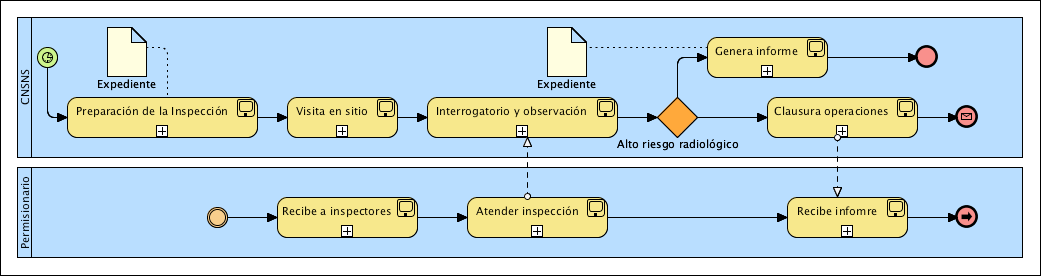
\includegraphics[width=.8\textwidth]{images/proceso2}
		\caption{PROC-02 Nombre del proceso}
		\label{fig:proceso2}
	\end{center}
\end{figure}

\begin{description}
	\item[Descripción:] ...
	\item[Entradas:] \cdtEmpty
        \begin{itemize}
			\item ...
        \end{itemize}
	\item[Salidas:] \cdtEmpty
        \begin{itemize}
			\item ...
        \end{itemize}	
    \item[Áreas de oportunidad:] Liste los aspectos que detecta se pueden mejorar con la introducción del sistema o los problemas encontrados.
\end{description}


%\input{proc/proc03.tex}
%\input{proc/proc04.tex}

%---------------------------------------------------------
\section{Modelo de procesos TO-BE}

Los nuevos procesos se presentan en esta sección, el mapa de procesos de se muestra en la figura~\ref{fig:mapaProc}.

\begin{figure}[htbp]
	\begin{center}
		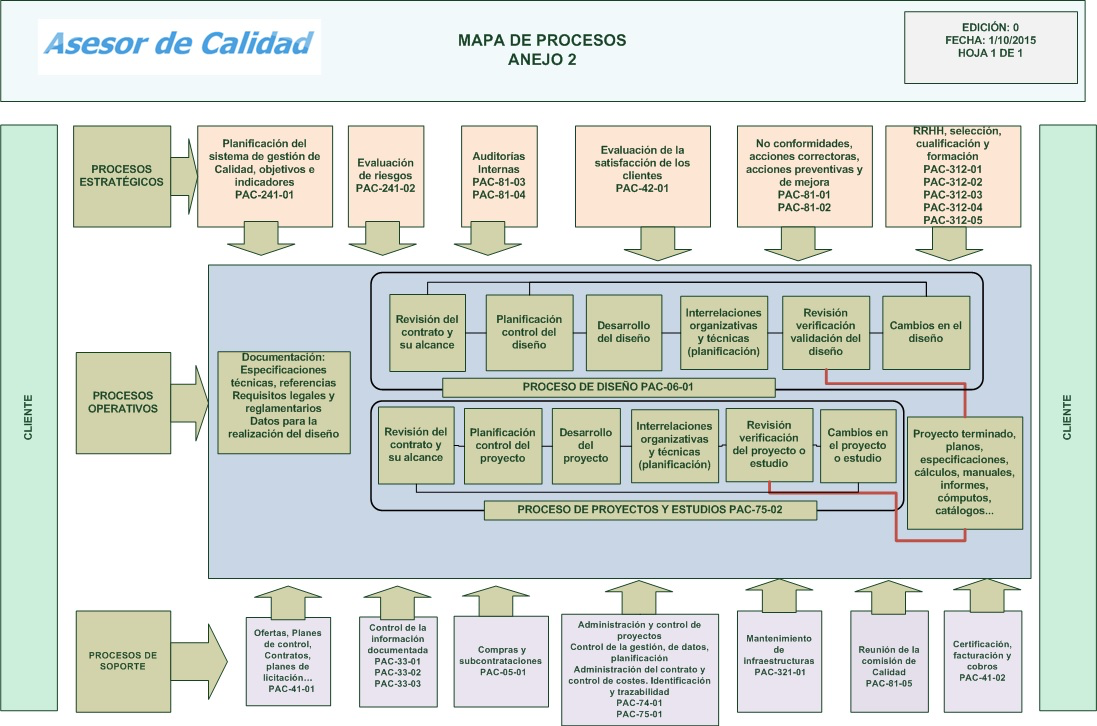
\includegraphics[width=.8\textwidth]{images/mapaProc}
		\caption{Mapa de procesos}
		\label{fig:mapaProc}
	\end{center}
\end{figure}


% - - - - - - - - - - - - - - - - - - - - - - - - - - - - 
\subsection{PROCM-01 ...}

\begin{figure}[htbp]
	\begin{center}
		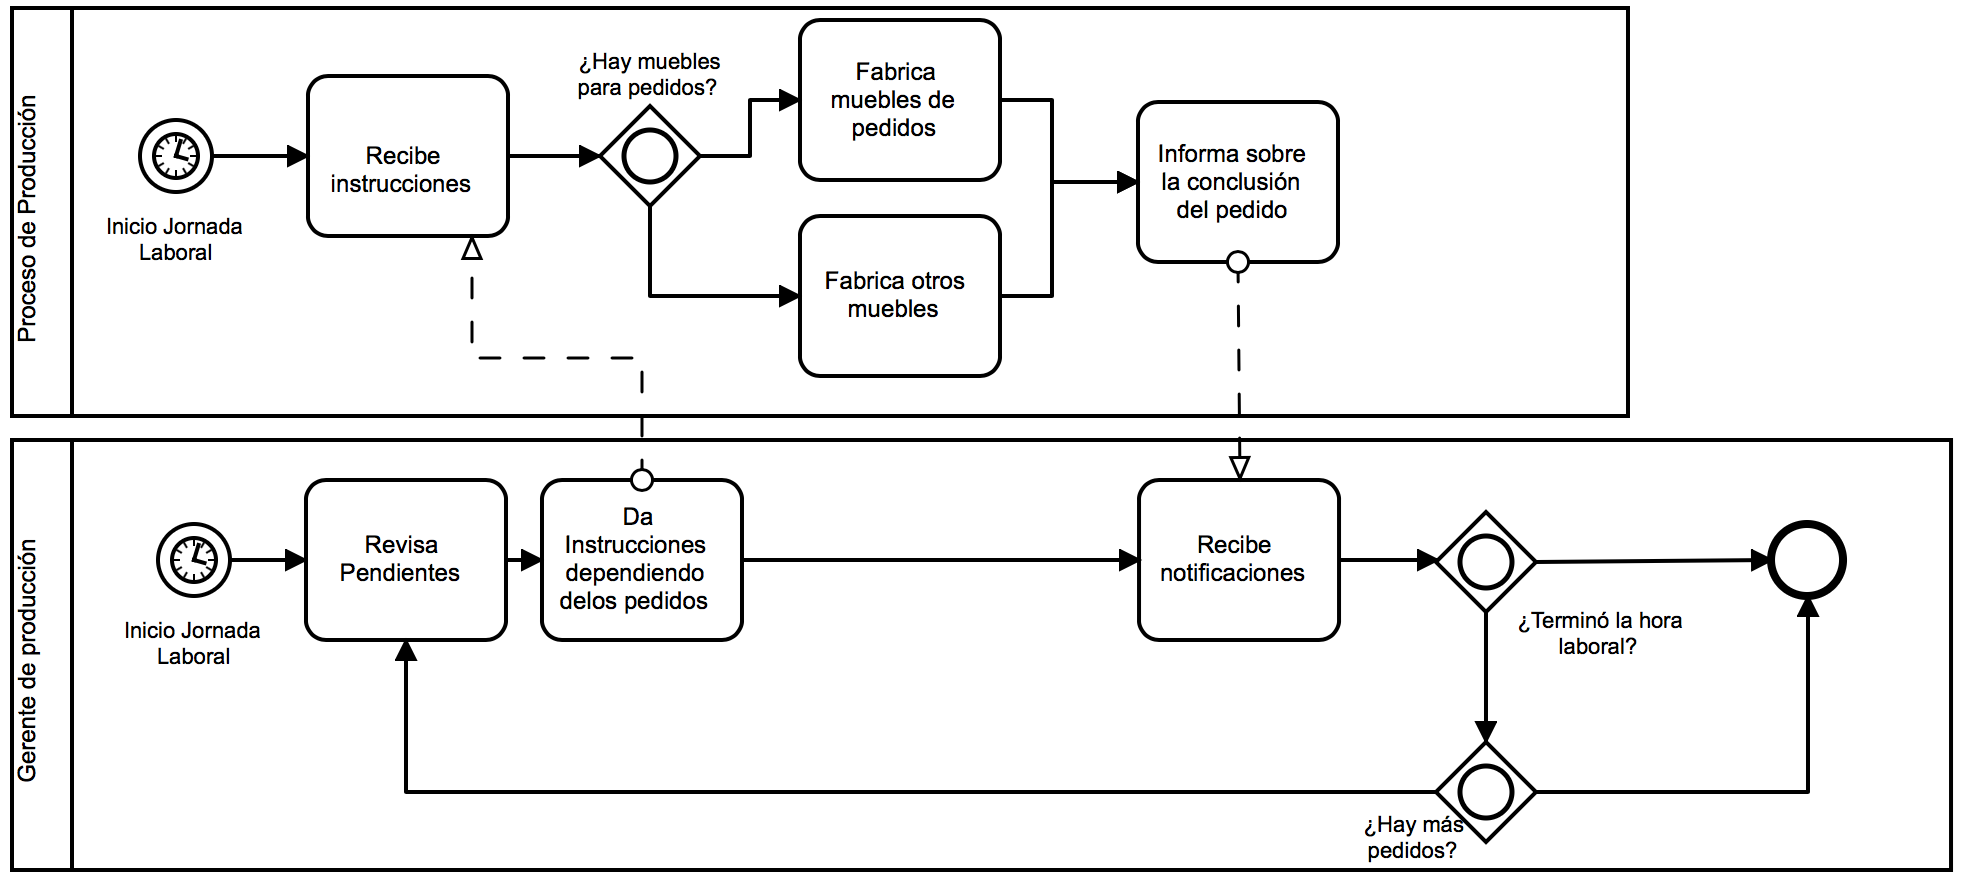
\includegraphics[width=.8\textwidth]{images/proceso3}
		\caption{PROCM-01 Nombre del proceso}
		\label{fig:proceso3}
	\end{center}
\end{figure}

\begin{description}
	\item[Descripción:] ...
	\item[Entradas:] \cdtEmpty
        \begin{itemize}
			\item ...
        \end{itemize}
	\item[Salidas:] \cdtEmpty
        \begin{itemize}
			\item ...
        \end{itemize}	
    \item[Mejoras esperadas:] Liste las mejoras que espera obtener tras la implementación del sistema.
    \item[Reglas de negocio:] \hyperlink{BR05}{BR05}, \hyperlink{BR8}{BR8}.
    \item[Casos de uso:] \hyperlink{CU3.4}{CU 3.4 Login}, \hyperlink{CU 4.3}{ CU 4.3 Consultar productos}.
\end{description}

%\input{proc/proc-m02.tex}
%\input{proc/proc-m03.tex}
%\input{proc/proc-m04.tex}


%
%%=========================================================
%%=========================================================
\chapter{Modelo dinámico}	
\label{cap:modDinamico}

	Este capítulo describe en modelo dinámico del sistema. en el se detallan todos los escenarios de ejecución del sistema. La figura~\ref{fig:casosDeUso} muestra el diagrama general del sistema y sus sib sistemas, y la figura~\ref{fig:casosDeUsoDetalle} muestra todos los casos de uso del sistema. En este documento solo detallamos los casos de uso del subsistema de gestión de cursos.
	
\begin{figure}[htbp]
	\begin{center}
		\fbox{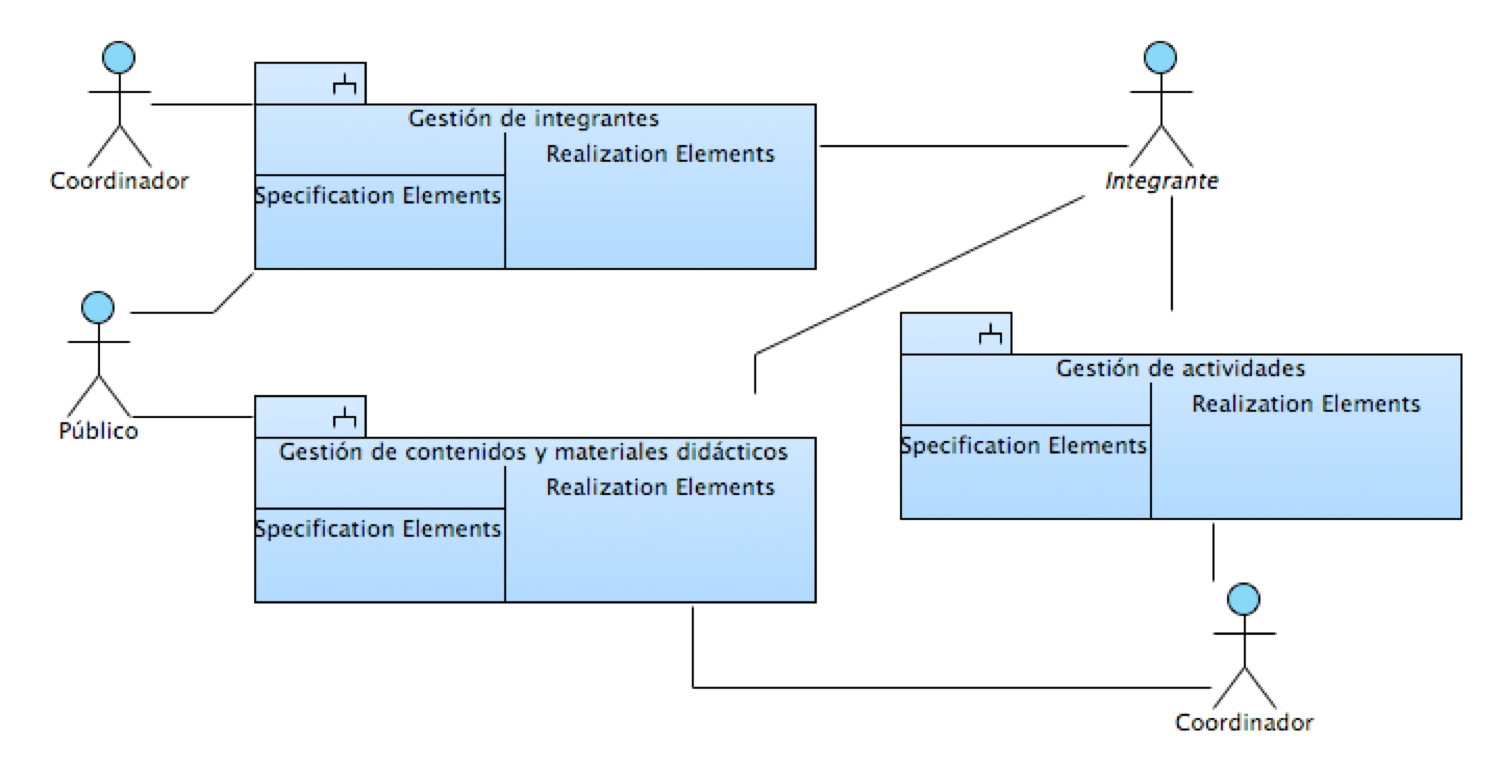
\includegraphics[width=.8\textwidth]{images/casosDeUso}}
		\caption{Diagrama de casos de uso del sistema.}
		\label{fig:casosDeUso}
	\end{center}
\end{figure}

\begin{figure}[htbp]
	\begin{center}
		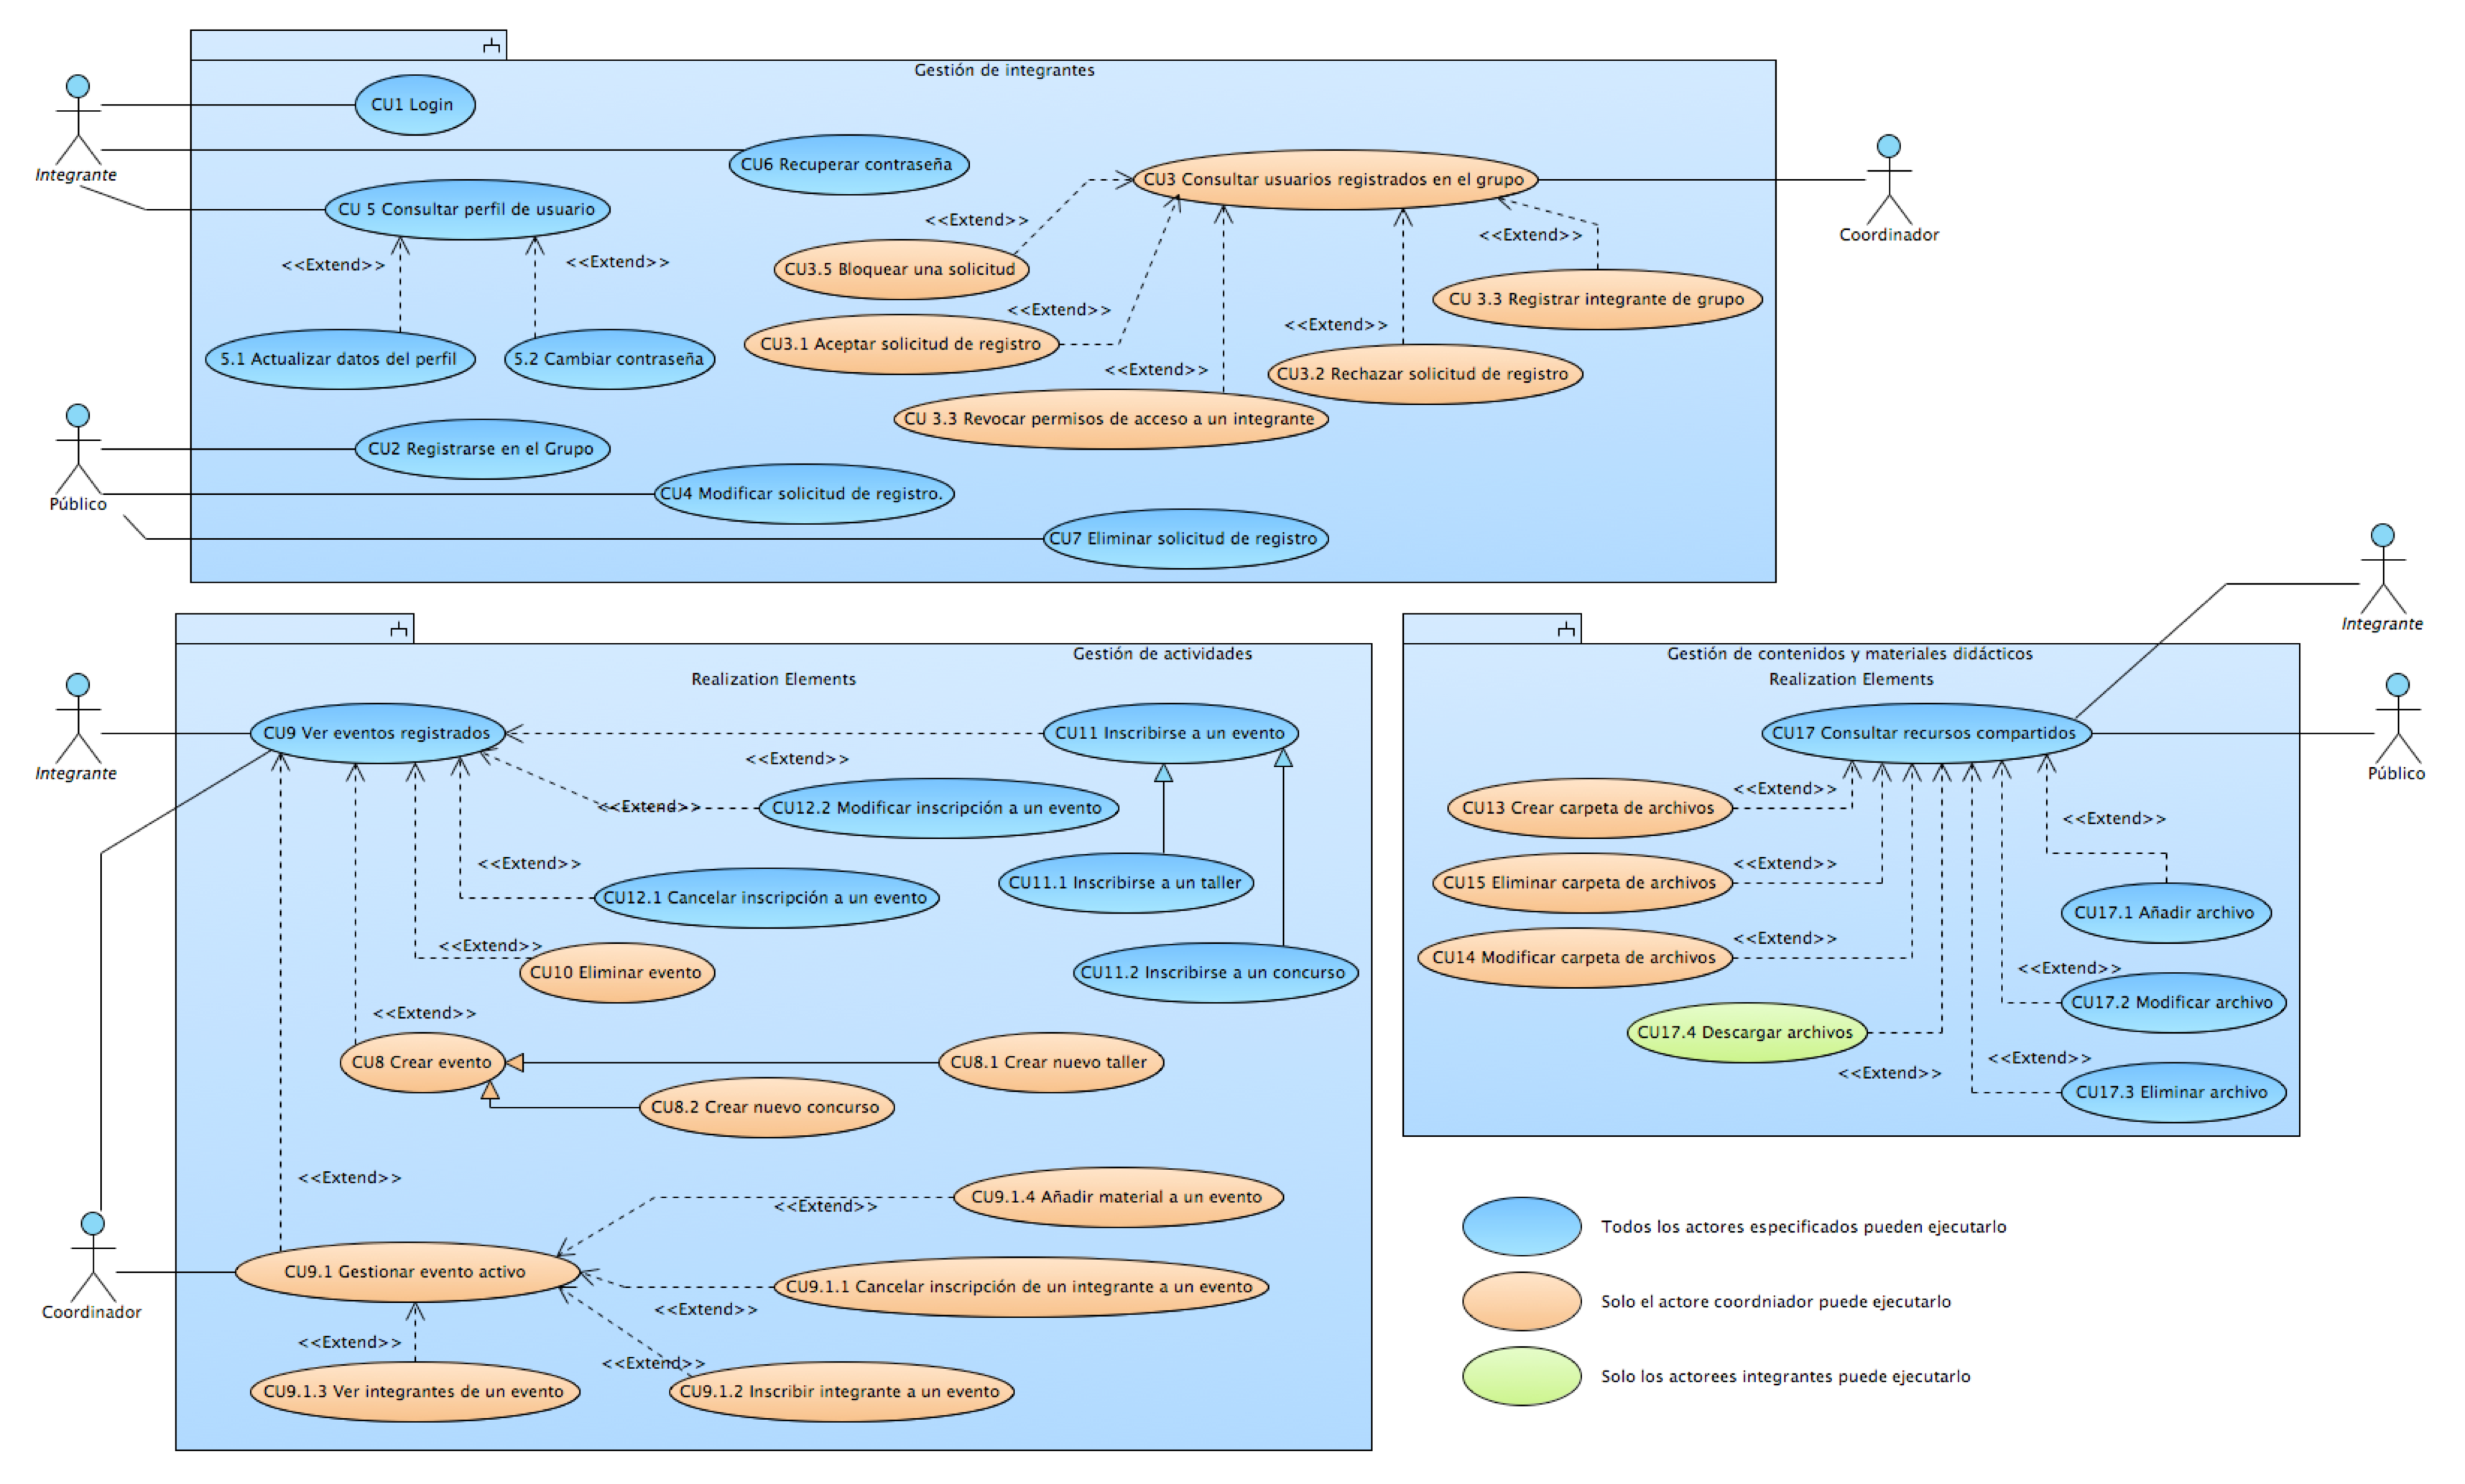
\includegraphics[angle=90, width=.7\textwidth]{images/casosDeUsoDetalle}
		\caption{Diagrama detallado del sistema.}
		\label{fig:casosDeUsoDetalle}
	\end{center}
\end{figure}

%---------------------------------------------------------
\section{Descripción de actores}

%---------------------------------------------------------
\begin{Usuario}{\hypertarget{getenteOperaciones}{\subsection{Gerente de Operaciones}}}{
	Es el encargado de todas las operaciones de la empresa y está por encima de los ejecutivos de producción y de ventas principalmente.
}
    \item[Responsabilidades:] \cdtEmpty
    \begin{itemize}
		\item Supervisar la operación.
		\item Plantear y supervisar el logro de las metas de la empresa y su crecimiento económico.
		\item ...
    \end{itemize}

	\item[Perfil:] \cdtEmpty
    \begin{itemize}
		\item Amplia experiencia en el ramo.
		\item Licenciatura como mínimo.
		\item ...
    \end{itemize}
\end{Usuario}

A continuación se detallan los casos de uso.

%---------------------------------------------------------
% CASOS DE USO

% \IUref{IUAdmPS}{Administrar Planta de Selección}
% \IUref{IUModPS}{Modificar Planta de Selección}
% \IUref{IUEliPS}{Eliminar Planta de Selección}

% 


% Copie este bloque por cada caso de uso:
%-------------------------------------- COMIENZA descripción del caso de uso.

%\begin{UseCase}[archivo de imágen]{UCX}{Nombre del Caso de uso}{
%--------------------------------------
	\begin{UseCase}{CU17}{Inscribir a Seminario}{
		Ayudar a que los Estudiantes que están por terminar la carrera se puedan inscribir en un Seminario de titulación.
	}
		\UCitem{Versión}{\color{Gray}0.1}
		\UCitem{Autor}{\color{Gray}David Ortega Pacheco}
		\UCitem{Supervisa}{\color{Gray}Ulises Vélez Saldaña.}
		\UCitem{Actor}{\hyperlink{Alumno}{Alumno}}
		\UCitem{Propósito}{Que el Estudiante se pueda inscribir a un seminario de titulación.}
		\UCitem{Entradas}{Número de boleta, Contraseña y Seminario.}
		\UCitem{Origen}{Teclado}
		\UCitem{Salidas}{Seminarios registrados, horario actual del Estudiante, desglose del monto a pagar por la inscripción, recibo de pago y comprobante de inscripción.}
		\UCitem{Destino}{Pantalla e impresora para recibo de pago y comprobante de inscripción}
		\UCitem{Precondiciones}{El estudiante debe estar registrado en la universidad.}
		\UCitem{Postcondiciones}{El estudiante quedará inscrito en el Seminario seleccionado si es elegible y hay cupo en el Seminario en cuestión.}
		\UCitem{Errores}{}
		\UCitem{Tipo}{Caso de uso primario}
		\UCitem{Observaciones}{}
	\end{UseCase}
%--------------------------------------
	\begin{UCtrayectoria}
		\UCpaso[\UCactor] Introduce su Número de Boleta y Contraseña en el sistema vía la  \IUref{IU23}{Pantalla de Control de Acceso}\label{CU17Login}.
		\UCpaso[\UCactor] Confirma la operación presionando el botón \IUbutton{Entrar}.
		\UCpaso Verifica que el Estudiante sea elegible para inscribirse al Seminario con base en la regla \BRref{BR129}{Determinar si un Estudiante puede inscribir Seminario.} \Trayref{A}.
		\UCpaso Despliega la \IUref{IU32}{Pantalla de Selección de Seminario} con la lista de Seminarios Disponibles.
		\UCpaso[\UCactor] Selecciona el Seminario en el que desea inscribirse \Trayref{B}\label{CU17SeleccionarSeminario}.
		\UCpaso Verifica que el Estudiante sea elegible para inscribirse al seminario seleccionado con base en la regla \BRref{BR130}{Determinar si un Estudiante puede inscribirse en un Seminario} \Trayref{C}.
		\UCpaso Verifica que el horario del Seminario concuerde con el horario del Estudiante con base en la regla \BRref{BR143}{Validar el horario del estudiante} \Trayref{D}.
		\UCpaso Calcula el costo del Seminario basado en el costo publicado en el catálogo de cursos, los costos aplicables al alumno y los impuestos aplicables, con base en las reglas \BRref{BR180}{Calcular costos del Estudiante} y \BRref{BR45}{Calcular impuestos por seminario}.
		\UCpaso Despliega el desglose de costos en la \IUref{IU33}{Pantalla Mostrar costos por seminario}.
		\UCpaso Pide al Estudiante que confirme la inscripción alSeminario.
		\UCpaso[\UCactor] Confirma la inscripción al Seminario.
		\UCpaso Inscribe al Estudiante en el Seminario seleccionado.
		\UCpaso Informa que la inscripción se realizó exitosamente vía la \IUref{UI88}{Pantalla de resumen de inscripción al Seminario}. 
		\UCpaso Imprime el recibo de pago con base en la regla \BRref{BR100}{Recibo del Estudiante por inscripción a Seminario.}.
		\UCpaso Pregunta al estudiante si desea imprimir un comprobante de la inscripción.
		\UCpaso[\UCactor] Indica que desea imprimir el comprobante de la inscripción.
		\UCpaso Imprime el comprobante de la inscripción \IUref{IU189}{Reporte de inscripción a Seminario}.		
	\end{UCtrayectoria}

%--------------------------------------		
		\begin{UCtrayectoriaA}{A}{El Estudiante no puede inscribir un Seminario}
			\UCpaso Muestra el Mensaje {\bf MSG1-}``El Estudiante [{\em Número de Boleta}] aun no puede inscribirse al seminario.''.
			\UCpaso[\UCactor] Oprime el botón \IUbutton{Aceptar}.
			\UCpaso[] Termina el caso de uso.
		\end{UCtrayectoriaA}
		
%--------------------------------------
		\begin{UCtrayectoriaA}{B}{El Estudiante abandona la operación}
			\UCpaso El Estudiante revisa la lista de Seminarios y no encuentra el Seminario que desea.
			\UCpaso[\UCactor] Oprime el botón \IUbutton{Salir}.
			\UCpaso Cierra la sesión del usuario.
			\UCpaso Continua en el paso \ref{CU17Login} del \UCref{CU17}.
		\end{UCtrayectoriaA}

%--------------------------------------
		\begin{UCtrayectoriaA}{C}{El estudiante no cumple con los prerrequicitos}
			\UCpaso Muestra el Mensaje {\bf MSG2-}``El Estudiante [{\em Número de Boleta}] no cumple con los requisitos para inscribirse al Seminario [{\em Nombre del Seminario seleccionado}].''.
			\UCpaso Muestra los requisitos que el Seminario seleccionado solicita.
			\UCpaso Continúa en el paso \ref{CU17SeleccionarSeminario} del \UCref{CU17}.
		\end{UCtrayectoriaA}

%--------------------------------------
		\begin{UCtrayectoriaA}{D}{El horario es incompatible.}
			\UCpaso Muestra el Mensaje {\bf MSG3-}``El horario del [{\em Nombre del Seminario seleccionado}] no es compatible con el horario del curso [{\em Nombre de la materia y grupo del curso con el que choca el horario}].''.
			\UCpaso Continúa en el paso \ref{CU17SeleccionarSeminario} del \UCref{CU17}.
		\end{UCtrayectoriaA}

%--------------------------------------
% Puntos de extensión
\subsection{Puntos de extensión}
\UCExtenssionPoint{
	% Cuando:
	Desea conocer las materias cursadas.
}{
	% Durante la región:
	Del paso 4 al paso 9.
}{
	% Casos de uso a los que extiende:
	\hyperlink{CU3.4}{CU3.4 Consultar historial académico}.
}
		
		
		
%-------------------------------------- TERMINA descripción del caso de uso.




%
%%=========================================================
%%=========================================================
\chapter{Modelo de la interacción}	
\label{cap:modInteraccion}

	Este capítulo describe ...

\section{Modelo de navegación}

	La navegación entre pantallas se muestra en la figura~\ref{fig:mapa}. en el se explica ...\\

\begin{figure}[htbp]
	\begin{center}
		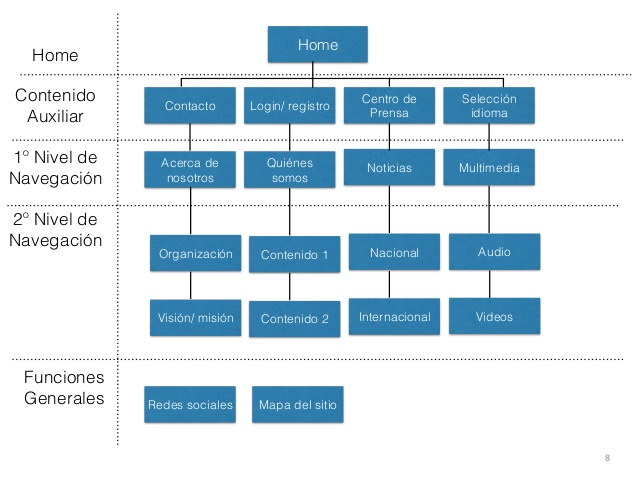
\includegraphics[width=.7\textwidth]{images/mapa}
		\caption{mapa}
		\label{fig:mapa}
	\end{center}
\end{figure}

%--------------------------------------
\section{IU23 Pantalla de Control de Acceso}

\subsection{Objetivo}
	Controlar el acceso al sistema mediante una contraseña a fin de que cada usuario acceda solo a las operaciones permitidas para su perfil.

\subsection{Diseño}
	Esta pantalla \IUref{IU23}{Pantalla de Control de Acceso} (ver figura~\ref{IU23}) aparece al iniciar el sistema. Para ingresar al mismo se debe escribir el Número de Boleta del estudiante y la contraseña de acceso. 

\IUfig[.5]{Login}{IU23}{Pantalla de Control de Acceso.}

\subsection{Salidas}

	Ninguna.

\subsection{Entradas}
Número de Boleta y Contraseña del Estudiante.

\subsection{Comandos}
\begin{itemize}
	\item \IUbutton{Entrar}: Verifica que el Estudiante se encuentre registrado y la contraseña sea la correcta. Si la verificación es correcta, se muestra la \IUref{UI32}{Pantalla de Selección de Seminario}.
	\item \IUbutton{Ayuda}: Muestra la ayuda de esta pantalla \IUref{IU50}{Pantalla de Ayuda}.
\end{itemize}

\subsection{Mensajes}

\begin{Citemize}
	\item Error al verificar los datos de acceso, vuelva a intentarlo.
\end{Citemize}





\printbibliography
\end{document}